% !TeX encoding = UTF-8
%% \textbf{重庆大学}通用毕业论文\LaTeXe{}模板
%%% 使用前请先阅读使用文档和用户协议,内有详细介绍。Happy Texing! :)
%% =======================================================
\documentclass%
	[type=doctor, bilinguallist=apart, printmode=twoside]{cquthesis}%
% 可用选项:
% type=[bachelor|master|doctor],      % 必选,毕业论文类型,以下项目不填时为默认
% liberalformat,                      % 可选,仅适用本科生,使用文学类论文标题格式,默认未打开
% proffesionalmaster=[true|false],    % 可选,仅适用研究生,是(true)否(false)专业硕士,默认为否
% printmode=[oneside|twoside|auto],	  % 可选,论文打印方式,默认采用auto按页数要求自动判定
% openany,|openright,                 % 可选,双面打印时每章的第一页仅右页开启,默认右页开启(openright)
% bilinguallist=[off|combined|apart], % 可选,图录表录等分别按双语题注混编(combined),分开编录(apart),默认关(off)
% blindtrail,                         % 可选,盲审模式,开启后封面姓名和致谢部分会隐藏,详情请参阅用户文档,默认关
% draft,                              % 写作期间可选,不渲染图片,关闭外围功能,加快预览速度,默认未开启

% 请在cquthesis.sty文件中定义其他会用到的宏包和自己的变量
% 这样可以防止main.tex太过臃肿。
\usepackage{cquthesis}

% 定义所有的图片文件在 figures 子目录下
\graphicspath{{figures/}}

% 定义数字圆
\usepackage{tikz}
\newcommand*\circled[1]{\tikz[baseline=(char.base)]{
            \node[shape=circle,draw,inner sep=1pt] (char) {#1};}}

%*** 写作时,使用这个命令只渲染你想查看的部分,提升工作效率,定稿时注释掉整行
%\includeonly{contents/experiment,contents/analysis,}

% 默认行间距 20 pt
\linespread{1.3}

\begin{document}

\cqusetup{
%	************	注意	************
%	* 1. \cqusetup{}中不能出现全空的行,如果需要全空行请在行首注释
%	* 2. 不需要的配置信息可以放心地坐视不理、留空、删除或注释(都不会有影响)
%	*
%	********************************
% ===================
%	论文的中英文题目
% ===================
  ctitle = {面向异构车联网的车载信息物理融合系统\\关键技术研究},
  etitle = {Research on Key Techniques for Vehicular Cyber-Physical Systems in Heterogeneous Vehicular Networks},
% ===================
% 作者部分的信息
% \secretize{}为盲审标记点,在打开盲审开关时内容会自动被替换为***输出,盲审开关默认关闭
% ===================
  cauthor = \secretize{许新操},	% 你的姓名,以下每项都以英文逗号结束
  eauthor = \secretize{Xincao~Xu},	% 姓名拼音,~代表不会断行的空格
  studentid = \secretize{},	% 仅本科生,学号
  csupervisor = \secretize{刘~~~~凯~~~~教授},	% 导师的姓名
  esupervisor = \secretize{{Prof.~Kai Liu}},	% 导师的姓名拼音
  cassistsupervisor = \secretize{}, % 本科生可选,助理指导教师姓名,不用时请留空为{}
  cextrasupervisor = \secretize{}, % 本科生可选,校外指导教师姓名,不用时请留空为{}
  eassistsupervisor = \secretize{}, % 本科生可选,助理指导教师或/和校外指导教师姓名拼音,不用时请留空为{}
  cpsupervisor = \secretize{}, % 仅专硕,兼职导师姓名
  epsupervisor = \secretize{},	% 仅专硕,兼职导师姓名拼音
  cclass = \rmfamily{2023}年\rmfamily{6}月,	% 博士生和学硕填学科门类,学硕填学科类型
  research_direction = \zihao{3}{车联网},
  edgree = {},	% 专硕填Professional Degree,其他按实情填写
% 提示:如果内容太长,可以用\zihao{}命令控制字号,作用范围:{}内
  cmajor = 工~~~~学,	% 专硕不需填,填写专业名称
  emajor = , % % 专硕不需填,填写专业英文名称
  cmajora = \zihao{3}{计算机科学与技术},
  cmajorb = \zihao{3}{车联网},
  cmajorc = \secretize{******~~~~教授},
%  cmajord = 2023年6月,
% ===================
% 底部的学院名称和日期
% ===================
  cdepartment = ,	%学院名称
  edepartment = ,	%学院英文名称
% ===================
% 封面的日期可以自动生成(注释掉时),也可以解除注释手动指定,例如:二〇一六年五月
% ===================
%	mycdate = {2023年6月},
%	myedate = {June 2023},
}% End of \cqusetup
% ===================
%
% 论文的摘要
%
% ===================
\begin{cabstract}	% 中文摘要

近年来,经济与社会不断发展,汽车的数量急剧增长,从而对人类社会与自然环境带来了诸多挑战。
随着感知技术、通讯方式与计算模式的发展,传统汽车正朝着智能化、网联化、协同化方向高速发展,以智能网联汽车为抓手,车联网驱动的智慧交通系统将有望于实现更加安全、高效、可持续发展的交通运输。
车联网中车载信息物理融合系统是实现智慧交通系统多样应用的基础和关键。
然而,车联网的固有特性和多元化的智能交通应用需求均给实现车载信息物理融合系统带来了巨大的挑战。
首先,面向高动态异构车联网,融合不同的计算范式与服务架构是实现车载信息物理融合的基础。
其次,面向分布式时变物理环境,有效的数据获取与建模评估是驱动车载信息物理融合的核心。
再次,面对动态异构节点资源,高效的任务调度与资源分配是进一步提升智慧交通系统服务质量的关键。
另外,面向多元智慧交通系统应用需求,满足差异性的系统质量与系统开销需求是驱动车载信息物理融合的另一关键。
最后,面向复杂的真实车联网环境,基于车载信息物理融合系统进行有效设计并实现具体系统原型是具有挑战的。

综上所述,本文从服务架构、评估指标设计、异构资源协同优化、质量-开销均衡和原型系统实现等五个方面对面向异构车联网的车载信息物理融合系统展开了研究。主要研究成果如下:

\circled{1} 基于软件定义网络和边缘计算的异构车联网架构研究。
首先,提出了面向下一代车联网的分层服务架构,旨在将软件定义网络和边缘计算范式在车联网中进行有机融合,并最大化其在信息服务方面的协同效应。
具体地,设计了一个四层架构,包括应用层、控制层、虚拟层和数据层,其目标是通过控制平面和数据平面的分离实现逻辑上的集中控制,基于网络功能虚拟化和网络切片促进自适应资源分配和面向服务的QoS,通过利用边缘计算服务的网络、计算、通信和存储能力来增强系统的可扩展性、响应性和可靠性。
其次,进一步分析了面临的新兴挑战,并通过提出跨层协议栈讨论了未来的研究方向。
最后,为了证明概念的可行性,在实际车联网环境中进行了两个案例研究。
现场测试结果不仅证明了所提服务架构的巨大潜力,还为未来智能交通系统的发展提供了启示。

\circled{2} 面向车载边缘计算的VCPS评估指标(Age of View)设计与优化策略研究。
首先,提出了面向车载边缘计算的协同感知和异质信息融合架构,其中边缘节点融合车辆协同感知的异构信息并构建逻辑视图。
其次,基于多类M/G/1优先队列建立了感知信息排队模型,并基于异质信息的时效性、完整性和一致性对车载信息物理融合质量进行建模。
具体地,设计了一个新颖的评估指标Age of View来定量衡量车载信息物理融合系统(VCPS)的质量。
再次,提出了一个基于差分奖励多智能体深度强化学习(MDR)解决方案。
特别地,系统状态包括车辆感知信息、边缘节点缓存信息和视图要求。
车辆动作空间包括信息感知频率和上传优先级。
边缘节点根据预测的车辆轨迹和视图需求分配V2I带宽给车辆。
最后,构建了仿真模型并进行了全面的性能评估,证明了MDR算法的优越性。

\circled{3} 面向NOMA车载边缘计算的异构资源协同优化策略研究。
首先,提出了基于NOMA的车载边缘计算架构,其通过异构边缘节点协同进行实时任务处理。
其次,通过考虑考虑了域内和域间的干扰建立了V2I传输模型,并形式化定义了通过联合任务卸载和资源分配的协同资源优化问题,旨在最大化服务率。
再次,将协同资源优化分解为两个子问题,即任务卸载和资源分配。
特别地,将任务卸载子问题建模为严格势博弈,并提出了多智能体分布式深度确定性策略梯度(MAD4PG)算法来实现纳什均衡。
资源分配子问题被分为两个独立的凸优化问题,并使用基于梯度的迭代方法和KKT条件提出了最优解。
最后,基于真实车辆轨迹构建了仿真模型,并进行了全面的性能评估,证明了MAD4PG算法的优越性。

\circled{4} 面向车载信息物理融合系统的质量-开销均衡优化策略研究。
首先,提出了车载信息物理融合架构,其中异质信息可以由车辆感知并通过V2I通信上传到边缘节点。
基于感知信息进行建模得到车联网中物理实体的数字孪生,并进一步构建逻辑视图以反映物理车联网环境的实时状态。
其次,建立了协同感知模型和V2I上传模型,并考虑数字孪生的时效性、一致性与冗余度,以及感知开销和传输开销,定义了VCPS质量和开销模型。
在此基础上,形式化定义了双目标问题,以最大化VCPS质量和最小化成本。
再次,提出了基于多智能体多目标深度强化学习(MAMO)的解决方案,其中提出了决斗评论家网络,基于状态价值和动作优势来评估智能体动作。
最后,进行了全面的性能评估,证明了MAMO算法的优越性。

\circled{5} 基于车载信息物理融合的超视距碰撞预警原型系统设计与实现。
首先,提出了超视距碰撞预警场景,其中车辆由于视线遮挡而具有潜在碰撞风险,而传统基于视距(LoS)的碰撞预警(例如,激光雷达、摄像头等)已不适用,因而进一步提出基于V2X通信的碰撞预警系统。
其次,提出了基于无线传输时延拟合模型与丢包检测机制的轨迹修正碰撞预警算法,通过丢包检测与时延补偿获得更加准确的车辆位置信息以构建更加精准的逻辑视图,以向超视距碰撞预警系统提供服务。
再次,建立了基于真实车辆轨迹的仿真实验模型并进行了全面性能评估,证明了所提碰撞预警算法的优越性。
最后,基于V2X的OBU和RSU设备,搭建了硬件在环与基于无人小车的试验平台,并在真实的车联网环境中,验证了所提算法的有效性。

\end{cabstract}
% 中文关键词,请使用英文逗号分隔:
\ckeywords{车载信息物理融合系统,异构车联网,评估指标设计,优化策略,深度强化学习}

\begin{eabstract}	% 英文摘要
Recently, with the continuous development of economy and society, the number of automobiles has increased dramatically, bringing many challenges to human society and the natural environment, such as traffic accidents, road congestion, and environmental pollution. 
With the development of sensing technology, communication methods, and computing paradigms, traditional vehicles are rapidly evolving towards intelligence, connected, and collaboration. 
Intelligent connected vehicles are driving the development of intelligent transportation systems (ITSs), which are expected to achieve safer, more efficient, and sustainable transportation.
In the vehicle-to-everything (V2X) communication network, the vehicular cyber-physical systems (VCPSs) is the foundation and key to realizing diverse ITS applications. 
However, the inherent characteristics of V2X and the diverse demands of ITS applications pose significant challenges to the implementation of such systems.
First, it is essential to combine different computing paradigms and service architectures for high-dynamic heterogeneous V2X to achieve VCPS. 
Second, effective data acquisition and modeling evaluation for distributed time-varying physical environments are the driving forces for VCPS. 
Third, efficient task scheduling and resource allocation are crucial for further improving the service quality of ITS in the face of dynamic heterogeneous resources. 
Fourth, to meet the diverse needs of ITS applications, satisfying the differentiated requirements of system quality and system overhead is another key factor driving VCPS. 
Finally, facing the complex real-world V2X environment, it is challenging to effectively design and implement specific system prototypes based on VCPS. 

This thesis conducts research on vehicular cyber-physical systems in heterogeneous vehicular networks from five aspects: service architecture, evaluation metric design, heterogeneous resource cooperative optimization, quality-cost tradeoff, and prototype system implementation. 
The main research contributions are as follows:

\circled{1} Research on the architecture of heterogeneous vehicular networks based on software-defined network and edge computing.
First, a hierarchical service architecture for the next generation of V2X is proposed to organically integrate software-defined networks and edge computing paradigms in vehicular networks, and maximize their synergistic effects on information services. 
Specifically, a four-layer architecture is designed, including the application layer, control layer, virtualization layer, and data layer. 
The goal is to achieve centralized control logically through the separation of the control plane and the data plane, promote adaptive resource allocation and service-oriented quality of service (QoS) based on network function virtualization and network slicing, and enhance the scalability, responsiveness, and reliability of the system by utilizing the network, computing, communication, and storage capabilities of edge computing services. 
Second, emerging challenges are further analyzed, and future research directions are discussed by proposing a cross-layer protocol stack. 
Finally, two case studies are conducted in actual V2X environments to demonstrate the feasibility of the proposed service architecture, providing insights for the development of future ITS.

\circled{2} Research on the evaluation metric (Age of view) design and optimization for VCPS in vehicular edge computing.
First, a cooperative sensing and heterogeneous information fusion architecture based on vehicular edge computing (VEC) is proposed, where edge nodes construct a logical view by fusing heterogeneous information sensed by vehicles collaboratively. 
Second, an information queuing model is established based on multi-class M/G/1 priority queues, and the quality of VCPS is modeled based on the timeliness, completeness, and consistency of heterogeneous information. 
A novel evaluation metric, Age of View, is designed to quantitatively measure the quality of VCPS. 
Third, a multi-agent difference-reward-based deep reinforcement learning (MDR) solution is proposed, where a difference reward (DR) based credit assignment scheme is designed to evaluate the contributions of individual vehicles on view construction; the edge node allocates V2I bandwidth to vehicles based on predicted vehicle trajectories and view requirements. 
Finally, a simulation model is constructed, and comprehensive performance evaluations are conducted, demonstrating the superiority of the proposed MDR algorithm.

\circled{3} Research on the cooperative optimization for heterogeneous resources in NOMA-based vehicular edge computing.
First, a non-orthogonal multiple access (NOMA) based architecture is proposed in VEC, where heterogeneous edge nodes are cooperated for real-time task processing. 
Second, a vehicle-to-infrastructure (V2I) transmission model is derived by considering both intra-edge and inter-edge interferences, and a cooperative resource optimization (CRO) problem is formulated by jointly optimizing the task offloading and resource allocation, aiming at maximizing the service ratio.
Third, the CRO is decomposed into two subproblems, namely, task offloading and resource allocation.
In particular, the task offloading subproblem is modeled as an exact potential game (EPG), and a multi-agent distributed distributional deep deterministic policy gradient (MAD4PG) is proposed to achieve the Nash equilibrium. 
The resource allocation subproblem is divided into two independent convex optimization problems, and an optimal solution is proposed by using a gradient-based iterative method and KKT condition. 
Finally, the simulation model is built based on real-world vehicular trajectories, and a comprehensive performance evaluation is given, which conclusively demonstrates the superiority of the proposed MAD4PG algorithm.
 
\circled{4} Research on quality-cost tradeoff optimization for VCPS.
First, a vehicular cyber-physical system architecture is proposed, in which heterogeneous information can be sensed by vehicles and uploaded to edge nodes via V2I communications. 
Based on the sensed information, digital twins of physical entities in the vehicular networks are modeled and further constructed into logical views to reflect the real-time state of the physical vehicular environment.
Second, a cooperative sensing model and V2I uploading model are established.
In particular, the VCPS quality and cost models are defined by considering the timeliness and consistency of digital twins, and the redundancy, sensing cost, and transmission cost,respectively. 
On this basis, a bi-objective problem is formulated to maximize the VCPS quality and minimize the VCPS cost.
Third, a solution based on multi-agent multi-objective deep reinforcement learning (MAMO) is proposed, in which a dueling critic network is proposed to evaluate agent actions based on the state value and action advantage.
Finally, a comprehensive performance evaluation is conducted, demonstrating the superiority of the proposed MAMO algorithm.

\circled{5} Design and implementation of a beyond-line-of-sight collision warning prototype system based on VCPS.
First, a beyond-line-of-sight collision warning scenario is proposed, in which vehicles have potential collision risks due to line-of-sight obstructions, and traditional line-of-sight (LoS) collision warning methods (such as LiDAR, cameras, etc.) are no longer applicable. 
Therefore, a collision warning system based on V2X communication is further proposed.
Second, a trajectory calibration collision warning algorithm based on a wireless transmission delay fitting model and packet loss detection mechanism is proposed. 
By using packet loss detection and delay compensation, more accurate vehicle position information is obtained to construct a more precise logical view to provide services for the beyond-line-of-sight collision warning system.
Third, a simulation experiment model based on real vehicle trajectories is established, and a comprehensive performance evaluation is given, demonstrating the superiority of the proposed collision warning algorithm.
Finally, based on V2X OBU and RSU devices, a hardware-in-the-loop and unmanned small vehicle-based test platform is set up, and the effectiveness of the proposed algorithm is verified in a real vehicular environment.
 
\end{eabstract}
% 英文关键词,请使用英文逗号分隔,关键词内可以空格:
\ekeywords{Vehicular cyber-physical systems, Heterogeneous vehicular networks, Metric design, Optimization method, Deep reinforcement learning
}

% 封面和摘要配置完成

\makecover %%% 封面部分


\frontmatter %%%前置部分(封面后绪论前)
%% 摘要
\makeabstract
%% 目录,注意需要多次编译才能更新
\tableofcontents
%% 插图索引,可选,如不用可注释掉
%\listoffigures
%\listoffiguresEN
%% 表格索引,可选
%\listoftables
%\listoftablesEN
%% 公式索引,可选
%\listofequations
%\listofequationsEN
%% 符号对照表,可选
%% !TeX encoding = UTF-8
% 环境用两个长度参数,分别定义左边距以及词条和解释的水平距离,可自己调试以达美观(全去掉时默认:20mm,30mm)
\begin{denotation}[20mm][15mm]
	\item[$\mathbf{T}$] 离散时间片集合 $\mathbf{T}=\{1, \ldots, t, \ldots, T\}$
	\item[$\mathbf{D}$] 异质信息集合 $\mathbf{D}=\{1, \ldots, d, \ldots, D\}$
	\item[$\operatorname{type}_d$] 信息$d$的类型
	\item[$u_d$] 信息$d$的更新时间间隔
	\item[$\left|d\right|$] 信息$d$的数据量
	\item[$\mathbf{V}$] 车辆集合 $\mathbf{V}=\{1, \ldots, v, \ldots, V\}$
	\item[$l_{v}^{t}$] 车辆$v$在时间$t$的位置
	\item[$\pi_{v}$] 车辆$v$的最大传输功率
	\item[$\mathbf{D}_v$] 车辆$v$感知信息集合
	\item[$\mathbf{K}_{v}$] 车辆$v$请求的任务集合
	\item[$d_{k}$] 任务$k$数据量
	\item[$c_{k}$] 任务$k$处理1 bit数据的CPU周期
	\item[$t_{k}$] 任务$k$处理截止时间
	\item[$\mathbf{E}$] 边缘节点集合 $\mathbf{E}=\{1, \ldots, e, \ldots, E\}$
	\item[$l_{e}$] 边缘节点$e$的位置
	\item[$b_{e}$] 边缘节点$e$的带宽
	\item[$g_{e}$] 边缘节点$e$的通信范围
	\item[$p_{e}$] 边缘节点$e$的最大功率
	\item[$c_{e}$] 边缘节点$e$的计算能力
	\item[$\mathbf{I}$] 视图集合 $\mathbf{I}=\{1, \ldots, i, \ldots, I\}$
	\item[$\mathbf{J}^{\prime}$] 车联网中物理实体集合 
	\item[$\mathbf{J}$] 数字孪生集合 
	\item[$\operatorname{dis}_{v, e}^{t}$] 车辆$v$与边缘节点$e$在时间$t$的距离
	\item[$n_{d, v}^t$] 0-1 变量指示车辆$v$在时间$t$是否感知信息$d$
	\item[$\lambda_{d, v}^{t}$] 车辆$v$在时间$t$对信息$d$的感知频率
	\item[$p_{d, v}^{t}$] 车辆$v$在时间$t$对信息$d$的上传优先级
	\item[$\pi_{v}^t$] 车辆$v$在时间$t$的传输功率
	\item[$b_{v, e}^{t}$] 边缘节点$e$在时间$t$为车辆$v$分配的带宽
	\item[$\pi_{v, e}^{t}$] 边缘节点$e$在时间$t$为车辆$v$分配的传输功率
	\item[$q_{v, e}^t$] 0-1 变量指示任务$k_v^t$是否卸载至边缘节点$e$
	\item[$c_{v, e}^t$] 边缘节点$e$在时间$t$为车辆$v$分配的计算资源
	\item[$\mathcal{G}$] 博弈模型
	\item[$\mathbb{S}$] 博弈策略空间
	\item[$\mathcal{S}$] 具体策略
	\item[$\mathbf{S}_{e}$] 边缘节点$e$的所有可能策略集合
	\item[$\mathcal{S}_{e}$] 边缘节点$e$的策略
	\item[$\mathcal{S}_{-e}$] 边缘节点 $e$ 的对手$\forall e^{\prime} \in \mathbf{E} \setminus \{e\}$所采取的联合策略
	\item[$\boldsymbol{o}^{t}$] 时间$t$的系统状态
	\item[$\boldsymbol{o}_{v}^{t}$] 车辆$v$在时间$t$对于系统状态的本地观测
	\item[$\boldsymbol{o}_{e}^{t}$] 边缘节点$e$在时间$t$对于系统状态的本地观测
	\item[$\boldsymbol{a}_{v}^{t}$] 车辆$v$在时间$t$的动作
	\item[$\boldsymbol{a}_{e}^{t}$] 边缘节点$e$在时间$t$的动作
	\item[$\boldsymbol{a}^{t}$] 智能体联合动作
	\item[$r^{t}$] 系统奖励
	\item[$r_{v}^{t}$] 车辆$v$在时间$t$的奖励
	\item[$r_{e}^{t}$] 边缘节点$e$在时间$t$的奖励
\end{denotation}

\endinput


\mainmatter %%% 主体部分(绪论开始,结论为止)
%* 子文件的多少和内容由你决定(最好以章为单位),基本原则是提速预览、脉络清晰、管理容易。


\chapter{绪\hskip\ccwd{}论}
\section{引言}\label{section 1-1}

随着国民经济和社会的高速发展,以及人们对美好生活的不懈追求,汽车已成为人们日常生活中不可或缺的交通工具之一。据统计,截至2021年底,我国民用汽车保有量高达30151万辆 \cite{gou2022zhong}。然而,汽车数量的急剧增长也给人类社会和自然环境带来了许多挑战。据世卫组织数据,全球每年约有130万人因道路交通事故死亡,另外约有2000至5000万人因事故受到非致命伤害,如致残等 \cite{shi2022dao}。同时,日益严峻的城市交通拥堵问题也给经济发展造成了巨大损失。此外,汽车也是空气污染物排放的主要贡献者之一,仅在2021年,全国汽车污染物排放总量就超过了1401.9万吨 \cite{shen2022zhong}。近年来,随着传感模式、通信技术和计算范式的发展,传统汽车正在向智能化、网联化和协同化方向迅猛发展。以智能网联汽车(Intelligent Connected Vehicle, ICV)为抓手,车联网(Vehicle-to-Everything, V2X)驱动的智能交通系统(Intelligent Transportation System, ITS)正致力于实现更加安全、高效和可持续发展的下一代交通运输。

近年来,车联网及其推动的智能网联汽车和智能交通系统已上升为我国的重要战略。2019年9月,国务院发布了《交通强国建设纲要》,提出要加强智能网联汽车的研发,通过新基建形成自主可控的车联网核心技术和生态产业链 \cite{zhong2019jiao}。2020年2月,国家发改委等11个部委联合发布了《智能汽车创新发展战略》,明确指出发展智能网联汽车对我国具有重要战略意义,并将突破关键核心技术作为首要战略任务 \cite{guo2020zi}。2022年8月,科技部发文支持建设包括智能港口、智能矿山和自动驾驶在内的十个新一代智能示范应用场景\cite{ke2022ke}。同时,车联网商业化也是业界关注的热点领域。2019年7月,华为发布了首款采用第五代移动通信(The 5th Generation Mobile Communication, 5G)技术的车载通信模组 MH5000,并与一汽、上汽、广汽等18家车企共同成立“5G汽车生态圈”,加速5G技术在汽车产业的商业进程。2020年10月,超过100家包括传统汽车制造商、芯片模组与硬件制造商、地图与定位服务提供商在内的相关企业,在中国上海开展了蜂窝车联网(Cellular-Vehicle-to-Everything, C-V2X)“新四跨”(跨芯片模组、跨终端、跨整车和跨安全平台)应用示范活动。截至2023年2月,已有包括一汽、上汽、广汽、通用、比亚迪和蔚来等十余家车企推出了C-V2X量产车型。

国内外许多一流高校和科研机构围绕车联网、车路协同、无人驾驶、智能交通系统等领域展开了深入探索与研究。清华大学汽车安全与节能国家重点实验室的李克强院士团队在智能网联汽车“中国方案”技术体系的提出和推动方面做出了重要贡献\cite{wang2023design, li2017dynamical, zheng2016stability}。中科院复杂系统管理与控制国家重点实验室的王飞跃院士团队在智能交通的信息物理融合方面取得了显著进展\cite{li2023sharing, liu2021cyber, lv2021guest}。无线移动通信国家重点实验室的陈山枝博士团队致力于C-V2X标准的制定和关键技术的研究,极大推动了车联网的产业化进程\cite{chen2023cellular, chen2020a, chen2017vehicle}。西安电子科技大学综合业务网理论与关键技术国家重点实验室的毛国强教授团队在车联网的高效数据分发、实时感知、ITS应用等方面取得了具有国际影响力的科研成果\cite{zhang2022new, hao2022dhcloc, yue2022towards}。深圳大学Victor C.M Leung(梁中明)教授团队专注于车联网边缘缓存、任务卸载和资源分配等领域的研究,并取得了系列重要科研成果\cite{sun2023federated, ju2023joint, wang2022efficient}。长安大学赵祥模教授团队在高速公路场景下智能车路协同体系架构以及相关运行安全性与适应性评估技术方面做出了重要贡献\cite{fang2022a, fang2022on, jing2022integrated}。

国际上,加拿大滑铁卢大学Sherman Shen(沈学民)教授团队在车联网安全\cite{chen2022adaptive}、车路协同\cite{liu2022real}和资源优化\cite{li2022cost}等领域取得了重要的研究突破。瑞典奥斯陆大学Yan Zhang(张彦)教授团队在车联网边缘计算\cite{dai2022adaptive}、内容缓存\cite{zhang2022digital}和资源分配\cite{sun2022dynamic}等领域取得了突出的贡献。香港理工大学Jiannong Cao(曹建农)教授团队在车联网边缘计算\cite{yang2022delegating}、计算卸载\cite{dai2023a}和数据分发\cite{yang2020efficient}等领域取得了重要的研究成果。澳大利亚悉尼大学Abbas Jamalipour教授团队在面向下一代网络中车联网通信\cite{qi2022energy}、感知\cite{iranmanesh2022a}和计算\cite{alam2022multi}等方面取得了重要的研究突破。美国休斯敦大学Zhu Han(韩竹)教授团队在车联网中安全\cite{khan2023federated}、无线资源分配\cite{zhang2023mean}以及博弈论应用\cite{kang2021joint}等领域展开了深入研究并取得了系列重要成果。加拿大卡尔顿大学F.Richard Yu(于非)教授团队在智能网联汽车中网络安全\cite{alladi2023ambient, liang2023a, bai2022detection}等领域进行了深入研究,并取得了重要的科研成果。香港理工大学Song Guo(郭嵩)教授团队在车联网边缘智能\cite{wang2922imitation, ren2021blockchain, wang2022design}等领域做出了突出贡献。日本东北大学Nei Kato教授团队在车联网中安全\cite{tang2020future}、智能反射面\cite{zhu2022intelligent}和边缘计算\cite{liu2020smart}等领域进行了全面深入的研究,并获得了系列重要科研成果。香港中文大学Guoliang Xing(刑国良)教授团队在自动驾驶\cite{he2021vi}和信息物理融合系统(Cyber-Physical System, CPS)\cite{shi2022vips}等领域取得了重要研究成果。

“信息物理融合系统”一词是由美国国家科学基金会的 Helen Gill 在2006年提出\cite{lee2016introduction}。自2011年Li等人\cite{li2011human}首次将信息物理融合系统应用于车联网中以来,车载信息物理融合系统(Vehicular Cyber-Physical System, VCPS)\cite{xia2019zi} 已成为国内外学术界热门的研究领域之一。车载信息物理融合系统利用智能网联汽车的多模态感知能力、V2X通信技术以及端边云的计算、存储和通信资源,形成一个集智能网联汽车、车联网、边缘计算、云计算等多种技术于一体的综合系统,并实现感知、计算、传输和控制的一体化。然而,车联网具有网络异构高动态、节点资源动态分布、ITS应用需求多元、真实环境复杂等特点,实现车载信息物理融合系统仍然面临巨大挑战。首先,未来车联网是一个多计算范式、服务架构共存的高动态网络,融合不同范式并最大化其协同效应,在此基础上,融合异质感知信息并评估其质量是 VCPS 的架构基础与驱动核心。其次,车联网中节点资源异构且受限,实现异构资源协同优化以最大化资源利用率是进一步优化 VCPS 服务质量的技术支持。再次,多元化ITS应用对VCPS的质量/开销需求具有差异性,实现VCPS质量-开销均衡是实现高质量低成本可扩展VCPS的理论保障。最后,在真实复杂性车联网通信环境中,设计和实现基于VCPS的典型应用是验证VCPS的必要手段。因此,本文将结合车联网高异构、高动态、分布式特征和智能交通系统的多样化应用需求,从架构融合与质量设计、异构资源协同优化、质量-开销均衡,以及原型系统实现方面进行理论、技术和系统上的综合创新。

\section{研究背景}\label{section 1-2}

本章节将首先介绍车联网的相关概念及其发展历程。接着,以智慧全息路口为例,介绍车载信息物理融合系统,并分析其中所面临的挑战。

\begin{figure}[h]
	\centering
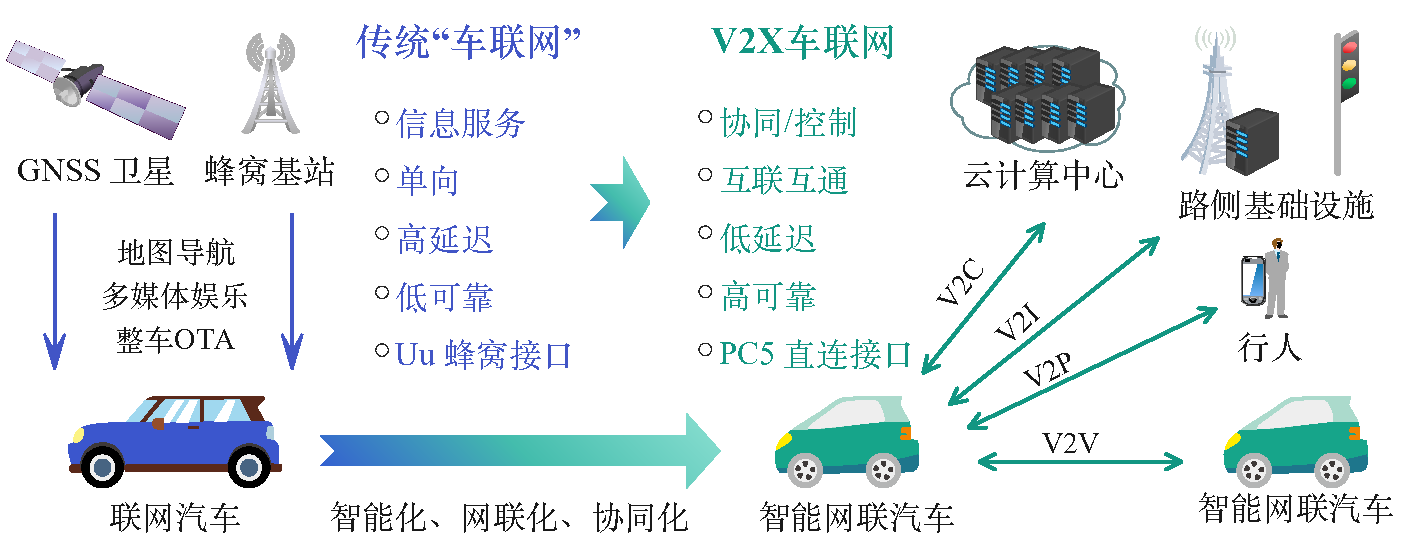
\includegraphics[width=1\columnwidth]{Fig1-1-V2X.pdf}
	\bicaption{从传统“车联网”到V2X车联网}{From traditional `connected cars' to V2X communications}
	\label{fig 1-1}
\end{figure}

车联网是物联网(Internet of Things, IoT)技术在汽车领域的应用形式。早在2G/3G移动网络时代,车联网已应用于利用全球导航卫星系统(Global Navigation Satellite System, GNSS)的定位信息为车辆提供防盗和救援服务。如今,智能网联汽车(如宝马、比亚迪、福特、通用、蔚来以及特斯拉等)都支持空中下载(Over-the-Air, OTA)技术对车机系统进行在线更新。如图 \ref{fig 1-1} 所示,随着汽车朝着智能化、网联化、协同化方向发展,传统的面向信息服务的“车联网”已经转变为与万物互联互通的V2X车联网。具体而言,V2X车联网是指多种通讯方式的融合,包括车辆间通讯(Vehicle-to-Vehicle, V2V)、车辆与行人通讯(Vehicle-to-Pedestrian, V2P)、车辆与基础设施通讯(Vehicle-to-Infrastructure, V2I)以及车辆与云端通讯(Vehicle-to-Cloud, V2C)。车联网利用实时数据分发,实现人、车、路等交通要素的协同配合,最终实现“聪明的车、智慧的路、协同的云”。此外,车联网还能促进基于单车智能的自动驾驶技术发展,通过车联网通信协助自动驾驶发现潜在危险,提升道路安全。随着我国车联网产业在政策规划、标准体系建设、关键技术研发、应用示范和基础设施建设等多方面的稳步发展,车联网的内涵和外延也在不断发展演进。依托快速落地的新型基础设施建设,车联网不仅广泛服务于智能网联汽车的辅助驾驶、自动驾驶等不同应用,还拓展服务于智慧矿山、智慧港口等企业生产环节以及智慧交通、智慧城市等社会治理领域\cite{zhong2021che}。

\begin{figure}[h]
	\centering
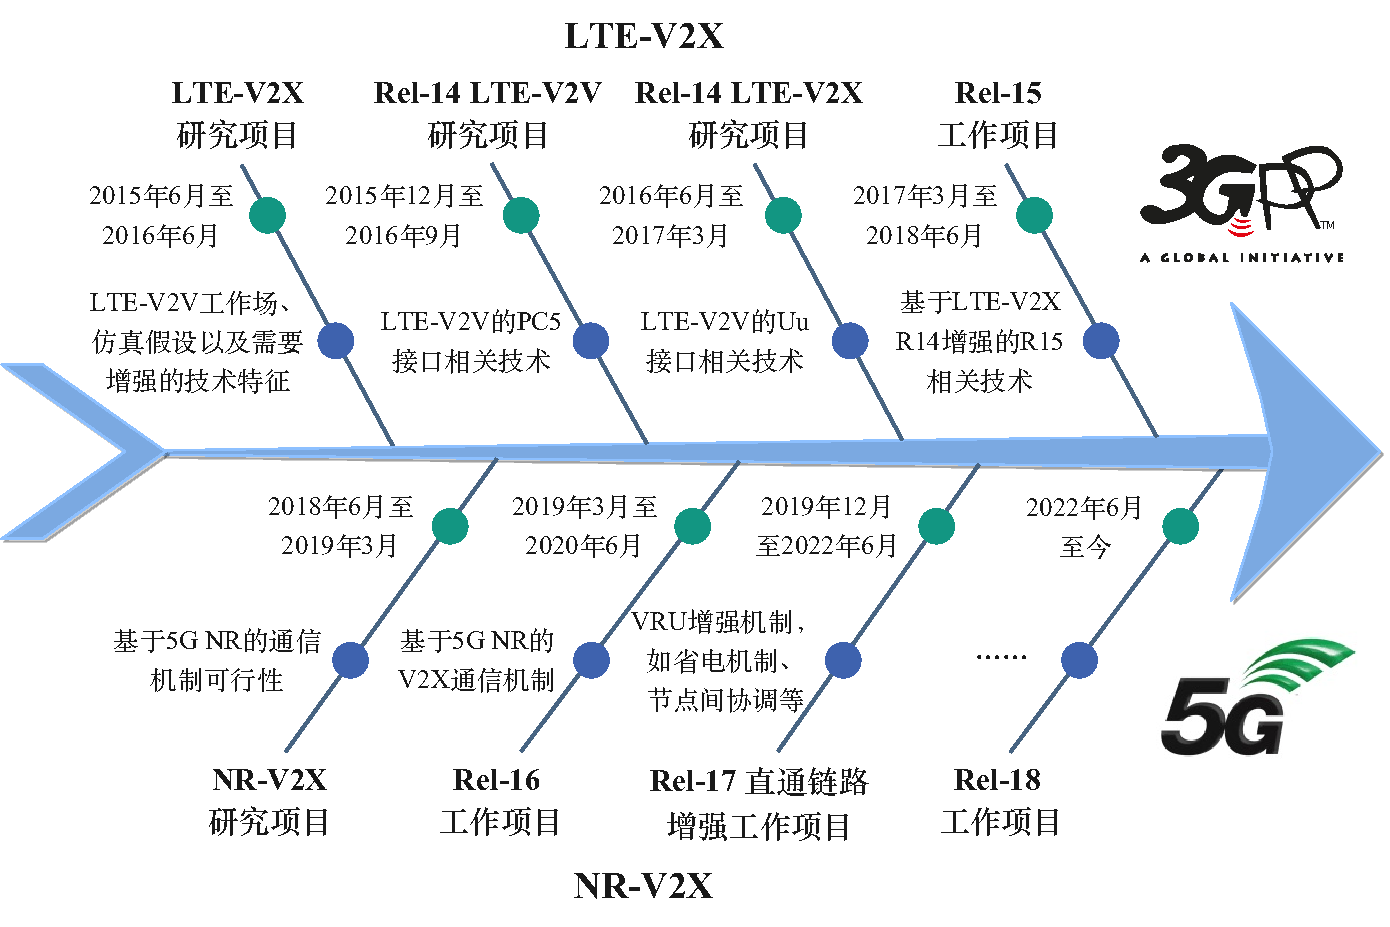
\includegraphics[width=1\columnwidth]{Fig1-2-V2X-evolution.pdf}
	\bicaption{3GPP C-V2X 标准演进}{3GPP C-V2X standard evolution}
	\label{fig 1-2}
\end{figure}

在车联网通信标准方面,电气和电子工程师协会(Institute of Electrical and Electronics Engineers, IEEE)在2003年提出了专用短距通信技术(Dedicated Short-Range Communication, DSRC)。2010年,IEEE发布了名为无线接入车载环境(Wireless Access in Vehicular Environments, WAVE)的协议栈,其中包括IEEE 802.11p、IEEE 1609.1/.2/.3/.4协议族和SAE J2735消息集字典 \cite{wu2013vehicular}。同时,基于长期演进(Long-Term Evolution, LTE)的V2X通信已形成一个完善的技术标准体系和产业链\cite{chen2016lte}。此外,IMT-2020(5G)推进组成立了C-V2X工作组,加速基于5G的V2X通信的演进。如图 \ref{fig 1-2} 所示,国际标准组织第三代合作伙伴计划(The 3rd Generation Partnership Project, 3GPP)在2018年启动基于5G新空口(New Radio, NR)的V2X标准研究,并在2020年完成了Rel-16版本的5G NR-V2X标准\cite{saad2021advancements},Rel-17版本进一步优化了功率控制、资源调度等相关技术。5G 汽车协会(5G Automotive Association, 5GAA)、下一代移动通信网络(Next Generation Mobile Network, NGMN)联盟以及5G Americas对IEEE 802.11p和C-V2X进行了技术对比,表\ref{table 1_1}显示C-V2X在传输时延、范围、速率以及可靠性等方面具有显著优势。目前,我国LTE-V2X产业蓬勃发展,与DSRC技术路线之争取得了重大进展。我国已建成基于LTE-V2X技术的完备产业链,芯片、模组、车载终端(Onboard Unit, OBU)、路侧设备(Roadside Unit, RSU)等均已成熟且经过了“三跨”“四跨”“新四跨”以及大规模测试,满足了商用部署条件。

\begin{table}[h]\small
\centering
\bicaption[C-V2X和IEEE 802.11p技术对比]{C-V2X和IEEE 802.11p技术对比\cite{cheng2021feng}}[Technical comparisons of C-V2X and IEEE 802.11p]{Technical comparisons of C-V2X and IEEE 802.11p \cite{cheng2021feng}}
\label{table 1_1}
\resizebox{\columnwidth}{!}{%
\begin{tabular}{@{}ccccc@{}}
\toprule
\begin{tabular}[c]{@{}c@{}}C-V2X\\ 技术优势\end{tabular} &
 \begin{tabular}[c]{@{}c@{}}具体技术\\ 或性能\end{tabular} &
IEEE 802.11p &
\begin{tabular}[c]{@{}c@{}}LTE-V2X\\ (3GPP R14/R15)\end{tabular} &
\begin{tabular}[c]{@{}c@{}}NR-V2X\\ (3GPP R16)\end{tabular} \\ \midrule
低时延 &
  时延 &
  不确定时延 &
  \begin{tabular}[c]{@{}c@{}}R14: 20ms\\ R15: 10ms\end{tabular} &
  3ms \\ 
\begin{tabular}[c]{@{}c@{}}低时延/\\ 高可靠\end{tabular} &
  \begin{tabular}[c]{@{}c@{}}资源分配\\ 机制\end{tabular} &
  CSMA/CA &
  \begin{tabular}[c]{@{}c@{}}支持感知+半持续\\ 调度和动态调度\end{tabular} &
  \begin{tabular}[c]{@{}c@{}}支持感知+半持续\\ 调度和动态调度\end{tabular} \\ 
\multirow{3}{*}[3.4ex]{高可靠} &
  可靠性 &
  不保证可靠性 &
  \begin{tabular}[c]{@{}c@{}}R14: \textgreater{}90\%\\ R15: \textgreater{}95\%\end{tabular} &
  支持99.999\% \\  
 &
  信道编码 &
  卷积码 &
  Turbo &
  LDPC \\ 
 &
  重传机制 &
  不支持 &
  \begin{tabular}[c]{@{}c@{}}支持HARQ,\\ 固定2次传输\end{tabular} &
  \begin{tabular}[c]{@{}c@{}}支持HARQ,\\ 传输次数灵活,\\ 最大支持32次传输\end{tabular} \\ 
\multirow{2}{*}[0ex]{\begin{tabular}[c]{@{}c@{}}更远传输\\ 范围\end{tabular}} &
  通信范围 &
  100m &
  \begin{tabular}[c]{@{}c@{}}R14: 320m\\ R15: 500m\end{tabular} &
  1000m \\  
 &
  波形 &
  OFDM &
  \begin{tabular}[c]{@{}c@{}}单载波频分复用\\ (SC-FDM)\end{tabular} &
  循环前缀(CP)-OFDM \\ 
\multirow{2}{*}[1.5ex]{\begin{tabular}[c]{@{}c@{}}更高传输\\ 速率\end{tabular}} &
  \begin{tabular}[c]{@{}c@{}}数据传输\\ 速率\end{tabular} &
  典型6Mbit/s &
  \begin{tabular}[c]{@{}c@{}}R14: 约30Mbit/s\\ R15: 约300Mbit/s\end{tabular} &
  \begin{tabular}[c]{@{}c@{}}与带宽有关,40MHz\\ 时R16单载波2层数据\\ 传输支持约400Mbit/s,\\ 多载波情况下更高\end{tabular} \\ 
 &
  调制方式 &
  64QAM &
  64QAM &
  256QAM \\ \bottomrule
\end{tabular}%
}
\end{table}

\begin{figure}[h] 
	\centering
	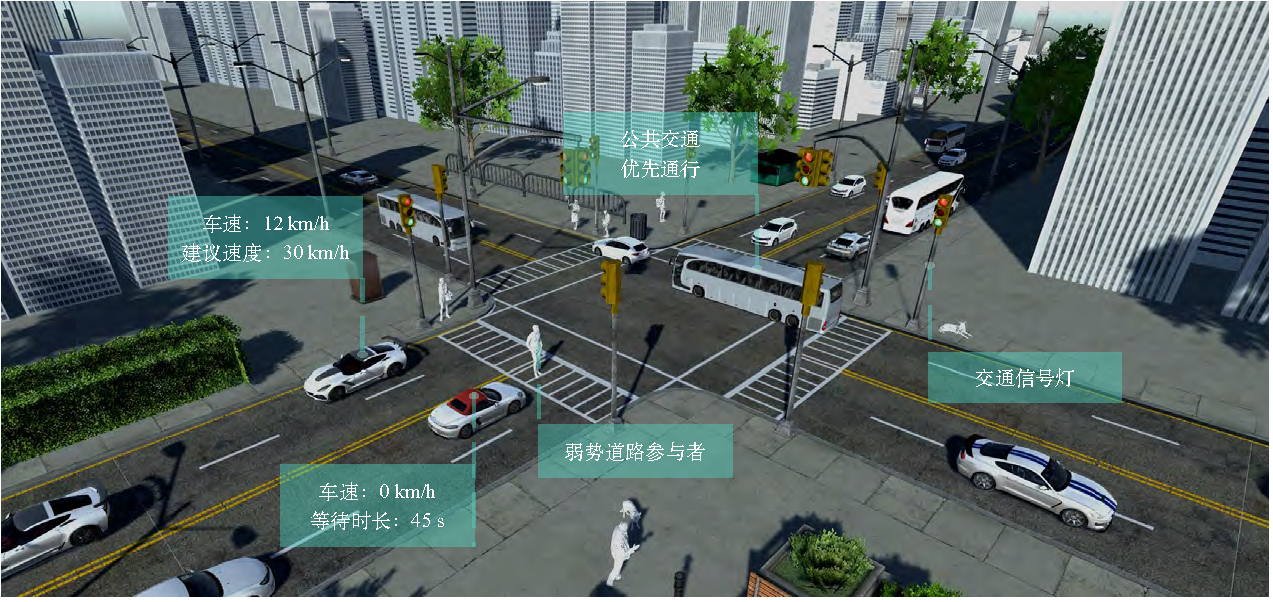
\includegraphics[width=1\columnwidth]{Fig1-3-intersection.pdf}
	\bicaption{基于车载信息物理融合的智慧全息路口}{Intelligent holographic intersection based vehicular cyber-physical fusion}
	\label{fig 1-3}
\end{figure}

如图 \ref{fig 1-3} 所示,智慧全息路口是一种基于车载信息物理融合技术的智慧交通管理系统。它通过将城市道路上的全要素进行数字化还原,为各类智能交通系统应用提供数据支撑。智慧全息路口利用道路基础设施和智能网联汽车上搭载的激光雷达、毫米波雷达、摄像头等多源传感设备,对路口进行全方位感知和全要素采集。通过传感设备实时感知交通流量、车速、车道变化等数据,并结合高精度地图呈现路口数字化上帝视角,精准刻画路口上的每一条车道、每一个交通信息灯的状态,以及每一辆车的行为轨迹。在实现路口全要素数字化还原的过程中,采用车载边缘计算技术将异构感知数据在边缘节点进行融合处理,从而提高数据处理速度,降低数据传输成本。同时,利用目标检测、目标跟踪、行为分析等算法对感知数据进行预处理,进一步提高数据准确性和精度,为后续的交通管理、交通安全和交通规划等应用提供更可靠的数据基础。

智慧全息路口不仅可以实现路口全要素数字化还原,而且可以进一步作为车载信息物理融合系统的外在展示和数据内核,支撑各种智能交通系统的应用。例如,全息路口可以为公交优先通行、绿波通行、弱势道路参与者(Vulnerable Road User, VRU)感知等 ITS 应用提供强有力的支持。在公交优先通行方面,全息路口可以根据公交车的实时位置和行驶速度,并结合路口的交通状况,提前调整信号控制策略,使公交车获得更好的通行效率和服务。在绿波通行方面,全息路口可以通过感知路口的交通流量和车速等信息,实现路口绿灯时长的自适应调整,从而实现车辆在绿波通信路段上的高效通行。在 VRU 感知方面,全息路口可以利用摄像头等传感设备或V2P通信感知VRU(如行人、自行车、残疾人等)的存在和行动轨迹,提供实时的路口状态信息和预警信息,保障弱势道路参与者的通行便利和交通安全。

通过以上讨论可知,车载信息物理融合系统是实现各类ITS应用的基础。然而,在高异构、高动态、分布式的车联网中,实现车载信息物理融合系统以满足多元ITS应用需求仍然面临着诸多问题和挑战。因此,针对以上问题和挑战,需要进一步展开全面深入的研究。具体地,首先,异构车联网亟需服务架构融合创新,并设计车载信息物理融合质量指标。未来车联网是一个多服务范式并存的高异构移动网络,因此需要研究异构车联网融合服务架构,以最大化不同服务范式的协同效应,并支持VCPS的部署实现。同时,现有研究都缺乏针对基于多源异质感知信息融合的VCPS进行整体深入的评估。因此,需要设计VCPS质量指标,并通过控制车辆感知行为与资源分配提升VCPS系统质量。其次,异构资源亟需协同优化。车联网中的通信和计算资源分布在不同的车辆和基础设施中,因此需要针对异构资源进行协同优化,支持VCPS中计算任务分布式处理,以进一步提升系统服务质量。再次,车载信息物理融合系统亟需质量-开销均衡优化。车载信息物理融合系统需要保证实时性和准确性的同时,考虑资源开销和能耗问题。因此,需要研究质量-开销均衡的优化策略,以提高系统的资源利用率的同时降低能耗。最后,亟需实现原型系统以验证VCPS性能。通过在真实车联网环境中搭建原型系统,可以进一步验证车载信息物理融合系统的可行性和有效性,为其在实际应用中提供更可靠的支持和保障。

\section{国内外研究现状}\label{section 1-3}

车载信息物理融合系统是实现各类智能交通系统应用的基础,其已成为国内外学术界研究的热点之一。本章节将对国内外相关研究工作进行梳理和总结,并从以下几个方面进行详细阐述:

\subsection{车联网服务架构研究与现状}

随着智能交通系统应用的不断涌现,传统车联网架构已无法满足大规模、高可靠、低时延的需求,因此研究人员正致力于将软件定义网络(Software Defined Network, SDN)新范式应用于车联网中。SDN通过分离数据平面和控制平面,实现了高度灵活的数据调度策略和网络功能虚拟化(Network Functions Virtualization, NFV)。Liu等人\cite{liu2016cooperative}首次将SDN概念应用于车联网中,提出了软件定义车联网(Software Defined Vehicular Network, SDVN),并在此基础上提出了基于混合V2I/V2V通信的在线协同数据调度算法,以提高数据分发的性能。Dai等人\cite{dai2018cooperative}设计了基于SDN的异构车联网中具有时间约束的时态信息服务调度方案。Luo等人\cite{luo2018sdnmac}提出了基于SDN的媒体接入(Media Access Control, MAC)协议以提高车联网的通信性能。Liu等人\cite{liu2018coding}提出了基于SDN的服务架构,并结合车辆缓存和网络编码来提高带宽利用率。Zhang等人\cite{zhang2022ac-sdvn}设计了一种解决SDVN中视频组播安全问题的安全访问控制协议,实现了多播视频请求车辆和RSU的身份认证。Zhao等人\cite{zhao2022elite}提出了一种基于智能数字孪生技术的软件定义车联网分层路由方案,克服了SDVN架构中高动态拓扑局限性。Lin等人\cite{lin2023alps}研究了一种基于SDVN的自适应链路状态感知方案,能够在信标间隔内及时获取链路状态信息,减少数据包丢失。Ahmed等人\cite{ahmed2023deep}提出了一个基于SDVN中车辆传感器负载均衡算法,并提出了一个数据包级入侵检测模型,可以跟踪并有效识别网络攻击。然而,现有大部分工作都仅是从数据分发、路由缓存、网络安全等方面展开了研究,缺乏对整体架构的深入分析。

移动边缘计算(Mobile Edge Computing, MEC)\cite{mao2017a}通过将计算、存储和网络资源靠近移动终端设备,提供更快速、更可靠的服务,同时减少网络流量消耗和服务延迟。越来越多的研究考虑将MEC范式应用在车联网环境中以提高系统实时性、可靠性和安全性。Liu等人\cite{liu2017a}首次将移动边缘计算融入车联网中,提出了车载边缘计算(Vehicular Edge Computing, VEC),并集成了不同类型的接入技术,以提供低延迟和高可靠性的通信。Lang等人\cite{lang2022cooperative}设计了一种基于区块链技术的协同计算卸载方案,以提高VEC资源的利用效率,并确保计算卸载的安全性。Liu等人\cite{liu2021fog}研究了端边云协同架构中的合作数据传播问题,并提出了一种基于Clique的算法来联合调度网络编码和数据分发。Dai等人\cite{dai2021edge}设计了一个基于自适应比特率多媒体流的VEC架构,其中边缘节点给以不同质量等级编码的文件块提供缓存和传输服务。Zhang等人\cite{zhang2022digital}提出了一种车载边缘缓存技术,动态调整边缘节点和车辆的缓存能力以提高服务的可用性。Liu等人\cite{liu2020adaptive}提出了一个两层的VEC架构,利用云、静态边缘节点和移动边缘节点来处理时延敏感性任务。Liao等人\cite{liao2021learning}研究了一种空地一体的VEC任务卸载策略,其中车辆能够学习具有多维意图的长期策略。Liu等人\cite{liu2023mobility}提出了一种利用车辆计算资源来提高VEC场景下任务执行效率的计算任务卸载方案。Liu等人\cite{liu2023asynchronous}研究了VEC中任务卸载和资源管理的联合优化问题,并采用异步深度强化学习算法来寻找最优解。然而,上述研究缺乏考虑异构车联网中不同服务架构的协同效应。

\subsection{车载信息物理融合系统质量指标研究与现状}

越来越多的研究人员聚焦于车载信息物理融合系统的预测、调度和控制技术,旨在有效提高 VCPS 系统的整体性能和可靠性。在预测技术方面,Zhang等人 \cite{zhang2021a} 提出了一种基于 VCPS 架构的车辆速度曲线预测方法,其协同 VCPS 中的不同控制单元来完成速度曲线预测。Albaba等人 \cite{albaba2021driver} 则结合深度Q网络(DQN)和层次博弈论,对高速公路驾驶场景中的驾驶员行为进行预测,其中k级推理被用来模拟驾驶员的决策过程。Zhang等人 \cite{zhang2020data} 提出了变道行为预测模型和加速预测模型。在此基础上,对车辆状态进行预测,并通过动态路由算法实现车辆之间的协同合作,以优化资源利用率和降低能源消耗。Zhou等人 \cite{zhou2021wide} 提出了一种基于宽-注意力和深度-组合模型用于交通流量预测。其中,宽-注意力模块和深度-组合模块分别用于提取全局关键特征和推广局部关键特征。在调度技术方面,Li等人 \cite{li2020cyber} 考虑了车辆移动性,并开发了一个基于物理比率-K干扰模型的广播方案,以确保通信的可靠性。Lian等人 \cite{lian2021cyber} 提出了一种基于既定地图模型路径规划的调度方法,以优化路径利用效率。在控制技术方面,Hu等人 \cite{hu2017cyber} 提出了一种燃油最优控制器,基于车队头车状态优化车辆速度和无级变速箱齿轮比。Dai等人 \cite{dai2016a} 提出了一种自主交叉路口控制机制,以确定车辆通过交叉路口的优先权。Lv等人 \cite{lv2018driving} 提出了一种自适应算法,用于三种典型驾驶方式下控制车辆加速。上述研究集中于支持 VCPS 的不同技术,如轨迹预测、路径调度和车辆控制等,虽然促进了各种 ITS 应用的实施,但是均建立在车联网中高质量物理元素建模信息可用的假设基础上,并未对车载信息物理融合质量进行定量分析。

部分研究工作侧重于利用深度强化学习(Deep Reinforcement Learning, DRL)优化 VCPS 中车辆感知和信息融合。Dong等人 \cite{dong2020spatio} 提出了一种基于 DQN 的方法,以融合在本地环境中获得的信息,从而做出可靠的车道变更决策。Zhao等人 \cite{zhao2020social} 设计了一个基于近似策略优化(Proximal Policy Optimization, PPO)的社会意识激励机制,以得出最佳的长期车辆感知策略。Mika等人 \cite{mlika2022deep} 提出了一个基于深度确定性策略梯度(Deep Deterministic Policy Gradient, DDPG)的解决方案,通过调度资源块和广播覆盖来优化信息时效性。然而,上述算法不能直接应用于 VCPS 中的协同感知和异构信息融合,并且,当考虑到多辆车场景时,上述算法并不适用。另一方面,部分研究对 VCPS 中的信息质量进行了评估。Liu等人 \cite{liu2014temporal} 提出了一种用于 VCPS 中时态数据传播的调度算法,其在实时数据传播和及时信息感知之间取得了平衡。Dai等人 \cite{dai2019temporal} 提出了一种进化多目标算法,以提高信息质量和改善数据到达率。Liu等人 \cite{liu2014scheduling} 提出了两种在线算法,通过分析传播特性来调度不同一致性要求下的时态数据传播。Rager等人 \cite{rager2017scalability} 开发了一个刻画真实网络随机性的框架,对随机数据负载进行建模以提高信息质量。Yoon等人 \cite{yoon2021performance} 提出了一个车联网中的合作感知框架,考虑到通信损耗和车辆随机运动,以获得车辆的精确运动状态。上述研究主要聚焦于 VCPS 中数据及时性、准确性或一致性方面的信息质量评估。然而,这些研究仅考虑了同质数据项层面的质量评估,没有针对车载信息物理融合进行质量评估。

\subsection{车联网资源分配与任务卸载研究与现状}

车联网中的资源分配一直是学术界的研究热点 \cite{noor-a-rahim2022a},大量研究人员针对车联网中通信资源分配进行了深入研究。He等人 \cite{he2022meta} 设计了一种动态车联网资源管理框架,其采用马尔可夫决策过程(Markov Decision Process, MDP)和分层强化学习相结合的方法,可以显著提高资源管理性能。Lu等人 \cite{lu2021user} 提出了一种基于用户行为的虚拟网络资源管理方法,以进一步优化车联网通信。Peng等人 \cite{peng2020deep} 提出了一种针对车联网的资源管理方案,通过应用 DDPG 方法解决了多维资源优化问题,实现了资源快速分配,并满足了车联网服务质量(Quality of Service, QoS)要求。Wei等人 \cite{wei2022multi} 针对车联网云计算中的资源分配问题,从提供者和用户双重视角出发,提出了一种改进的 NSGA-II 算法来实现多目标优化。Peng等人 \cite{peng2021multi} 研究了无人机辅助车联网中的多维资源管理问题,并提出了一种基于多智能体深度确定性策略梯度(Multi-Agent Deep Deterministic Policy Gradient, MADDPG)的分布式优化方法,实现了车辆资源联合分配。为了进一步提高频谱利用率和支持更多车辆接入,部分研究将非正交多址接入(Non-Orthogonal Multiple Access, NOMA)技术融入车联网中。Patel等人 \cite{patel2021performance} 评估了基于 NOMA 的车联网通信容量,其数值结果显示,NOMA 通信容量比传统的正交多址接入(Orthogonal Multiple Access,OMA)高出约20\%。Zhang等人 \cite{zhang2021centralized} 利用基于图的匹配方法和非合作博弈(Non-Cooperative Game,NCG)分布式功率控制,为NOMA车联网开发了一个集中的两阶段资源分配策略。Zhu等人 \cite{zhu2021decentralized} 提出了一种考虑随机任务到达和信道波动的最优功率分配策略,以最大化长期的功率消耗和延迟。Liu等人 \cite{liu2019energy} 在基于 NOMA 的车联网中,提出了基于交替方向乘子法(Alternating Direction Method of Multipliers,ADMM)的功率分配算法。然而,上述研究主要是基于单边缘节点的情况,无法处理不同边缘节点之间的相互干扰情况。因此,仍然需要探索更加复杂的多边缘节点环境下的资源分配策略,以提高车联网的性能和可靠性。


随着车载边缘计算的发展,大量研究专注于 VEC 中的任务卸载和资源分配。其中,Liu等人\cite{liu2021rtds}提出了一种多周期任务卸载的实时分布式方法,通过评估 VEC 中的移动性感知通信模型、资源感知计算模型和截止时间感知奖励模型。Shang等人\cite{shang2021deep}研究了节能的任务卸载,并开发了一种基于深度学习的算法来最小化能耗。为了最小化执行延迟、能源消耗和支付成本的加权和,Liu等人\cite{liu2022a}提出了一种结合 ADMM 和粒子群优化(Particle Swarm Optimization, PSO)的任务卸载算法。Chen等人\cite{chen2020robust}设计了一种带有故障恢复功能的计算卸载方法,以减少能源消耗并缩短服务时间。为了实现超高可靠低时延通信(ultra-Reliable and Low-Latency Communication, uRLLC)服务需求下最大化吞吐量,Pan等人\cite{pan2022asynchronous}提出了一种基于异步联合 DRL 的计算卸载方案。Zhu等人\cite{zhu2022a}提出了一种用于智能反射面(Intelligent Reflecting Surface, IRS) 辅助下的 VEC 的动态任务调度算法,优化有限资源分配并考虑了车辆的移动模式、传输条件和任务大小以及并发传输之间的相互干扰。此外,部分研究聚焦于采用多智能体强化学习(Multi-Agent Deep Reinforcement Learning, MADRL)算法的任务卸载和资源分配。Alam等人\cite{alam2022multi}开发了一种基于 DRL 的多智能体匈牙利算法,用于 VEC 中的动态任务卸载以满足延迟、能耗和支付费用需求。Zhang等人\cite{zhang2021adaptive}提出了一种基于 MADDPG 的边缘资源分配方法,在严格延迟约束下最小化车辆任务卸载成本。为了同时满足严格延迟要求和最小带宽消耗,He等人\cite{he2021efficient}提出了一种多智能体行动者-评论家(Multi-Agent Actor-Critic, MAAC)算法,用于车辆带宽分配。然而,以上研究工作都没有考虑实时任务卸载和通信/计算资源分配的协同优化。

部分研究专注于VEC的联合通信和计算资源分配。Cui等人\cite{cui2021reinforcement}提出了一种多目标的强化学习方法,通过协同通信和计算资源的分配来减少系统延迟。Han等人\cite{han2020reliability}设计了基于动态规划(Dynamic Programming,DP)的资源分配方法,实现了耦合车辆通信和计算资源的可靠性计算。Xu等人\cite{xu2021socially}采用契约理论为每个潜在的内容供应商和内容请求者分配通信和计算资源。少数研究者研究了联合任务卸载和资源分配。Dai等人\cite{dai2021asynchronous}提出了一个异步的DRL算法,实现了异构服务器数据驱动的任务卸载。此外,Dai等人 \cite{dai2022a}开发了一种概率计算卸载方法,根据边缘节点的计算分配概率进行计算卸载的独立调度。Nie等人\cite{nie2021semi}提出了一种MADRL算法,在无人机辅助VEC中联合优化资源分配和功率控制。然而,现有研究主要基于集中式调度,通信开销和调度复杂性较高,不适用于大规模的车联网。

\subsection{车载信息物理融合中质量/开销优化研究与现状}

近年来,许多研究人员致力于提高车载信息物理融合中的 QoS,以提升 ITS 应用的用户体验。其中,Wang等人\cite{wang2016offloading}提出了一种组合优化方法,旨在减少移动数据流量的同时满足 VCPS 中面向 QoS 的服务需求。Jindal等人\cite{jindal2018sedative}提出了一种基于 SDN 和深度学习的 VCPS 网络流量控制方案,成功解决了网络流量管理问题。Zhu等人\cite{zhu2022joint}设计了一种基于双时间尺度 DRL 的方法,以优化基于车辆编队的 VCPS 中的车辆间距和通信效率,同时满足 V2I 通信的 QoS 要求。Wang等人\cite{wang2023a}提出了一种集群式车辆通信方法,通过公交车聚类和混合数据调度实现了从公交车到普通车辆的有效数据传播并满足了严格和个性化的 QoS 需求。此外,Chen等人\cite{chen2021qos}致力于解决 IRS 辅助车联网中的频谱共享问题,通过优化车辆的发送功率、多用户检测矩阵、频谱重用以及 IRS 反射系数等参数,提高车联网通信的服务质量。Lai等人\cite{lai2017a}提出了一种基于 SDN 的流媒体传输方法,根据用户移动信息、播放缓冲区状态和当前网络信号强度向 SDN 控制器提供流媒体传输策略,以实现最小延迟和更好的 QoS。Tian等人\cite{tian2022multiagent}则设计了一种基于 MADRL 的资源分配框架,以共同优化信道分配和功率控制,满足车联网中的异构 QoS 需求。同时,Zhang等人\cite{zhang2020hierarchical}研究了 MEC 车联网中联合分配频谱、计算和存储资源问题,并利用 DDPG 解决该问题,以满足 ITS 应用的 QoS 要求。Sodhro等人\cite{sodhro2020ai}建立了可靠和延迟容忍的无线信道模型和多层边缘计算驱动的框架,有效提升了车联网服务质量。

另一方面,部分研究人员致力于降低 VCPS 中的各类开销。例如,Zhao等人\cite{zhao2021a}设计了一种基于 SDN 和无人机(Unmanned Aerial Vehicle, UAV)辅助的车辆计算卸载优化框架,其中采用了UAV辅助车辆计算成本优化算法以最小化系统成本。Zhang等人\cite{zhang2019hybrid}提出了一种基于蚁群优化和三个变异算子的算法,用于优化具有灵活时间窗口的多目标车辆路径,以最小化行驶成本和车辆固定成本。Ning等人\cite{ning2020when}则针对5G车联网中无线频谱有限的问题,构建了一个智能卸载框架,联合利用蜂窝频谱和未许可频谱来满足车辆需求,并在考虑时延限制的基础上使成本最小化。Tan等人\cite{tan2019twin}提出了一种基于人工智能(Artificial Intelligence,AI)的多时间尺度框架的联合通信、缓存和计算策略,其中考虑了车辆的移动性和硬服务截止期限约束,并实现了最大化网络成本效益。Hui等人\cite{hui2022collaboration}提出了一种协作自动驾驶方案,并通过联盟博弈机制来确定最佳车辆分簇,以最小化每个簇的计算成本和传输成本。虽然上述研究对 VCPS 系统中的开销进行了深入研究,但这些研究并未考虑车载信息物理融合系统构建的质量和开销。因此,需要进行对 VCPS 系统本身的评估与质量-开销均衡的深入研究。

\subsection{智能交通系统安全相关应用研究与现状}

随着城市化进程的加速和交通流量的不断增加,ITS 安全相关应用的部署可以大幅提高道路交通的安全性。因此,许多研究人员针对驾驶员状态监测、驾驶行为分析、交通监测等方面进行了研究。Mugabarigira等人\cite{mugabarigira2023context}提出了一种基于车辆行为追踪和驾驶风险分析的导航系统,可提高城市道路上车辆的安全性。Chang等人\cite{chang2018design}提出了一种基于可穿戴智能眼镜的疲劳驾驶检测系统,能够实时检测驾驶员的疲劳或嗜睡状态。Dutta等人\cite{dutta2022design}提出了一种基于凸优化的鲁棒分布式状态估计系统,可保护连接车辆的传感器数据免受拒绝服务(Denial-of-Service, DoS)或虚假数据注入(False Data Injection, FDI)攻击。Wang等人\cite{wang2021deep}提出了一种基于深度学习加速器嵌入式平台的鲁棒雨滴检测系统,并利用检测结果自动控制汽车雨刷。Sun等人\cite{sun2022toward}提出了一种有效的交通估计系统,可通过与过往车辆通信并记录其出现情况来实现自动交通测量,为ITS提供关键信息。

部分研究工作从车辆控制、车辆编队控制、路口交通流控制等多个层面对 ITS 安全相关应用展开了深入分析。Zhang等人\cite{zhang2021data}提出了一种分布式安全巡航控制系统,利用历史数据建立了车辆行为预测模型和动态驾驶系统模型,并设计了考虑合并行为概率的安全跟驰控制策略。Zhao等人\cite{zhao2022resilient}提出了一个具有鲁棒性的车辆编队控制系统,并设计了一种在多重干扰和 DoS 攻击下恢复机制,降低 DoS 攻击对 VCPS 的不利影响。Pan等人\cite{pan2023privacy}设计了一种面向车联网的车队隐私保护集结控制系统,通过采样数据的动态加密和解密方案,使得车队之间的通信数据得以保密。Li等人\cite{li2021confidenitality}介绍了一种低延迟协作安全车辆编队数据传输系统,采用无线电信道相关性的协作密钥协商协议以保证数据传输的安全。Kamal等人\cite{kamal2021control}提出了一种多智能体路口交通流控制系统,利用随机梯度方法计算交通信号灯持续时间。Lian等人\cite{lian2021cyber}提出了基于交通控制的智能物流系统,并设计了改进的A*路径规划算法以实现主动调度和碰撞避免。

作为典型 ITS 安全相关应用,车辆碰撞预警已引起广泛研究人员的关注。目前,大多数车辆碰撞预警系统都是基于超声波雷达或激光雷达等测距传感器的。Song等人\cite{song2018real}提出了一种实时障碍物检测和状态分类方法,该方法融合了立体摄像头和毫米波雷达,并结合车辆运动模型,通过多个模块感知环境,能够准确快速地判断出“潜在危险”物体。Wu等人\cite{wu2019series}提出了一种77GHz车辆碰撞预警雷达系统短程天线,该系统采用补丁阵列天线作为基本结构,并采用多层板设计技术使其尺寸更小。然而,这些方案都存在非视距(Non-Line-Of-Sight, NLOS)的问题,即在障碍物遮挡情况下基于视距(Line-Of-Sight, LOS)的方法不再适用。近年来,随着计算机视觉的发展,一些研究集中在基于摄像头实时视频流的碰撞检测上。Wang等人\cite{wang2016vision}提出了一种新颖的车辆制动行为检测方法,利用安装在挡风玻璃上的摄像头来捕获前车信息,以避免与前方车辆相撞。Song等人\cite{song2018lane}提出了一种轻量级的基于立体视觉的车道检测和分类系统,以实现车辆的横向定位和前向碰撞预警。然而,基于计算机视觉的方法需要大量数据传输和密集计算,这使得系统的性能无法得到实时响应。另一方面,部分研究考虑了通过 V2X 通信实现碰撞预警。Hafner等人\cite{hafner2013cooperative}基于 V2V 通信技术实现了一种分布式算法,用于交叉路口的车辆协同防撞。Gelbar等人\cite{gelbal2017elastic}提出了一个基于 V2X 通信的车辆碰撞预警和避免系统。然而,无线通信中的传输时延和数据包丢失等内在特征是不可避免的,对于车辆碰撞预警系统也是不可忽视的。这使得在真实复杂车联网环境中实现实时和可靠的安全关键型服务变得更加困难。

\section{研究目标与研究内容}\label{section 1-4}

\subsection{研究目标}

本文针对异构车联网高动态物理环境、动态分布式车联网节点资源、智能交通系统多元应用需求,以及真实复杂性车联网通信环境所带来的挑战,从架构融合与指标设计、协同资源优化、质量-开销均衡,以及原型系统实现四个方面对车载信息物理融合系统展开研究。本文的研究目标如下:

\circled{1} 针对车联网高异构、高动态、高分布式等特征,提出融合软件定义网络和移动边缘计算的车联网分层服务架构,并实现视图质量的量化评估,是车载信息物理融合系统的架构基础与驱动核心。首先,结合软件定义网络、网络功能虚拟化和网络切片等关键思想,提出车联网分层服务架构,以支持 VCPS 的部署与实现。其次,提出基于多类 M/G/1 优先队列的感知信息排队模型。进一步,针对边缘视图对于感知信息的时效性、完整性以及一致性需求,设计 VCPS 质量指标,并形式化定义视图质量优化问题。最后,提出基于差分奖励的多智能体强化学习视图质量优化策略,实现高效实时的边缘视图构建。

\circled{2} 针对车联网中异构节点资源、动态拓扑结构与无线通信干扰等特征,实现基于边缘协同的异构资源优化,是进一步优化 VCPS 服务质量的技术支撑。首先,面向 NOMA 车联网的车载边缘计算环境,考虑 V2I 通信中边缘内与边缘间干扰,提出 V2I 传输模型,并考虑边缘协作提出任务卸载模型。其次,形式化定义协同资源优化问题,并将其分解为任务卸载与资源分配两个子问题。最后,提出基于博弈理论的多智能体强化学习算法的资源优化策略,具体地,基于多智能体强化学习实现任务卸载博弈的纳什均衡,并基于凸优化理论提出最优资源分配方案,实现最大化资源利用效率。

\circled{3} 针对多元智能交通系统应用对于视图质量/开销的差异性需求,实现车载信息物理融合质量-开销均衡,是实现高质量低成本车载信息物理融合的理论保障。首先,考虑视图中信息的及时性与一致性需求,建立车载信息物理融合质量模型。其次,考虑视图构建中感知信息的冗余度、感知开销与传输开销,建立车载信息物理融合开销模型。最后,提出基于多目标多智能体强化学习的质量与开销均衡策略,实现高质量低成本可扩展车载信息物理融合。

\circled{4} 针对真实复杂性车联网通信环境中验证车载信息物理融合的需求,设计并实现基于车载信息物理融合的原型系统,是验证车载信息物理融合的必要手段。首先,提出基于视图修正的碰撞预警算法。其次,搭建基于 C-V2X 设备的硬件在环测试平台,实现硬件在环性能验证。最后,在真实车联网环境中,实现基于车载信息物理融合的超视距碰撞预警原型系统,进一步验证所提算法和系统模型的可行性和有效性。

\subsection{研究内容}

本文致力于研究车载信息物理融合系统,主要研究内容及关系如图 \ref{fig 1-4} 所示。
首先,面向异构车联网高动态物理环境,融合不同的计算范式与服务架构,并实现有效的数据获取与建模评估是车载信息物理融合的架构基础与驱动核心。
因此,本文将首先研究如何设计融合软件定义网络和移动边缘计算的车联网分层服务架构,在此基础上,研究如何评估并提高车载边缘侧所构建的逻辑视图质量。
其次,面向动态分布式车联网节点资源,高效的任务调度与资源分配是车载信息物理融合的技术支撑。
因此,本文将研究如何实现异构资源协同优化,提高资源利用效率。
面向多元智能交通系统应用需求,实现车载信息物理融合质量-开销均衡是车载信息物理融合的理论保障。
因此,本文将进一步研究车载信息物理融合质量/开销模型及其均衡优化策略。
最后,面向真实复杂性车联网通信环境,基于车载信息物理融合设计并实现具体系统原型是车载信息物理融合的验证手段。
因此,本文将更进一步设计及实现基于车载信息物理融合的超视距碰撞预警原型系统,实现理论与系统的相互促进。
本文具体研究内容如下:

\begin{figure}[h] 
	\centering
	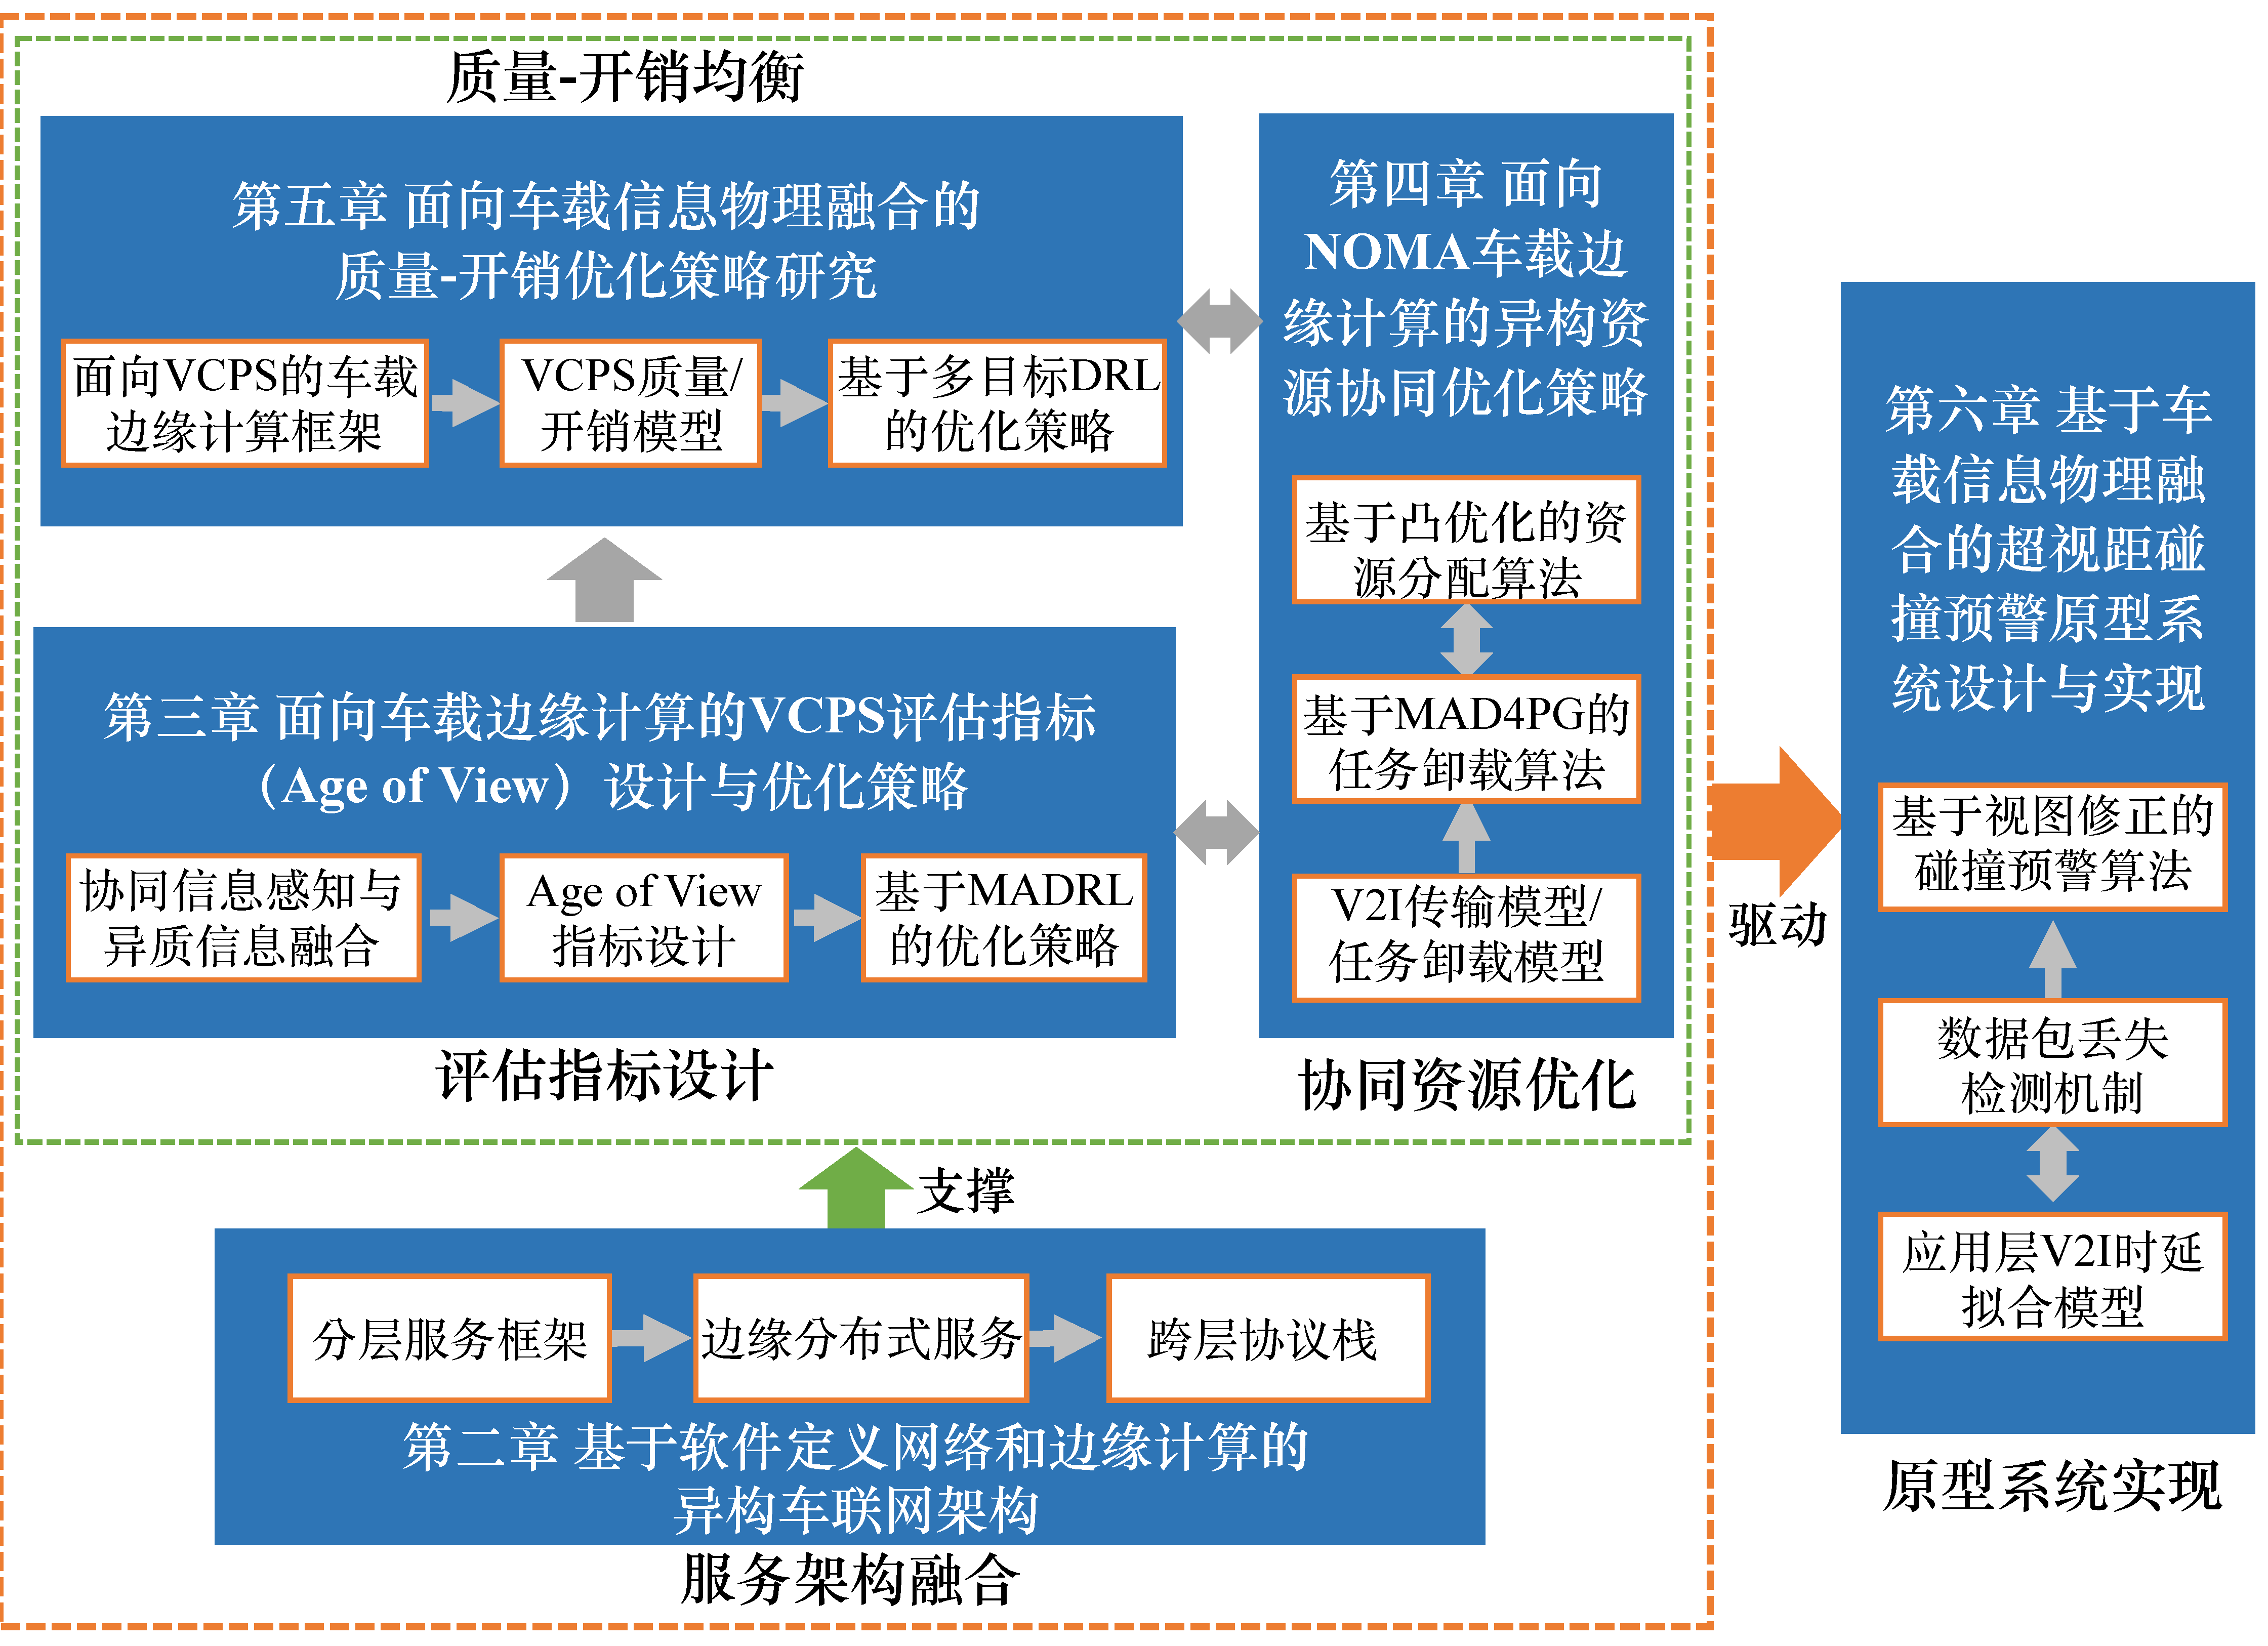
\includegraphics[width=1\columnwidth]{Fig1-4-content.pdf}
	\bicaption{主要研究内容}{Main research content}
	\label{fig 1-4}
\end{figure}

\circled{1} 基于分层车联网架构的车载信息物理融合质量指标设计与优化。
考虑车联网环境中的网络资源的高异构性、车联网物理环境分布式时变性、拓扑结构的高动态性,以及车辆节点感知能力差异性等关键特征,本文将研究融合软件定义网络和移动边缘计算的分层车联网服务架构。进一步,本文将重点研究基于分层服务架构的分布式感知与异质信息融合模型,考虑信息的多维需求,研究车载信息物理融合质量指标设计。在此基础上,研究基于差分奖励多智能体强化学习的边缘视图优化策略。

\circled{2} 面向车载信息物理融合的通信与计算资源协同优化关键技术。
考虑车联网高动态环境与高异构分布式资源,本文将引入NOMA技术提升车联网频谱资源利用效率,并提出基于边缘协同的异构资源优化策略。本文将重点研究 V2I 传输与任务卸载模型,并在此基础上,研究基于博弈理论多智能体深度强化学习的异构资源协同优化策略,具体地,基于凸优化理论,研究通信资源最优分配策略,并基于任务卸载势博弈模型,研究基于多智能体深度强化学习的任务卸载算法。

\circled{3} 面向车载信息物理融合的质量-开销均衡优化关键技术。
考虑智能交通系统中多元应用需求,本文将研究车联网中不同交通要素的视图质量与开销模型,并提出车载信息物理融合质量-开销均衡优化策略。本文将综合考虑视图的建模质量,包括信息的及时性与一致性,研究车载信息物理融合质量模型,并考虑视图的构建开销,包括信息冗余度、感知开销与传输开销,研究车载信息物理融合开销模型。在此基础上,研究基于多目标多智能体深度强化学习的车载信息物理融合质量-开销均衡优化策略。

\circled{4} 面向车载信息物理融合系统的超视距碰撞预警原型系统设计与实现。
考虑真实复杂性车联网通信环境,本文将研究基于车载信息物理融合系统的超视距碰撞预警原型系统设计与实现。具体地,本文将研究C-V2X应用层时延拟合模型和数据丢包检测机制,并研究基于视图修正的碰撞预警算法。在此基础上,研究基于 C-V2X 通信设备的硬件在环试验平台搭建方案,并研究在真实车联网环境中基于车载信息物理融合的超视距碰撞预警原型系统实现方案。

\section{论文的特色与创新之处}\label{section 1-6}

区别于目前仅专注于车联网通信协议、服务架构、资源分配和智能应用等方面的研究,本文旨在从实际需求出发,分析当前面临的挑战,并在车载信息物理融合系统的四个方面进行深入研究:架构基础与驱动核心、技术支撑、理论保障与验证手段。本文的具体特色在于:
a) 针对异构车联网高动态物理环境和信息感知的时效性与准确性需求,考虑到感知信息时变性、车辆节点移动性和感知能力差异性所带来的挑战,研究如何将基于SDN的集中控制和基于移动边缘计算的分布式调度有机结合,并在边缘侧建立有效的逻辑视图,为车载信息物理融合系统提供架构基础和驱动核心。
b) 针对动态分布式车联网节点资源,考虑节点异构资源的动态性、分布性和无线通信中边缘内和边缘间干扰所带来的挑战,研究如何实现边缘协同,最大化异构资源利用效率,为车载信息物理融合系统提供技术支撑。
c) 针对多元智能交通系统的应用需求,考虑到车联网中不同交通要素视图质量和开销需求差异所带来的挑战,研究如何实现车载信息物理融合系统的质量-开销均衡,为车载信息物理融合系统提供理论保障。
d) 针对真实复杂的车联网通信环境,考虑基于真实C-V2X通信设备部署和实现原型系统所带来的挑战,研究基于车载信息物理融合的超视距碰撞预警系统的原型设计和实现,为车载信息物理融合系统提供系统验证。
本文的主要创新点概括如下:

\circled{1} 提出融合软件定义网络与移动边缘计算的车联网分层服务架构,并定义边缘视图概念,率先设计视图评估指标并建立视图质量评估模型,提出分布式信息感知与异质信息融合的边缘视图构建机制:现有车联网服务架构相关研究主要关注于单一范式的实践应用,难以适用于具有大规模数据服务需求的下一代车联网场景与支撑车载信息物理融合系统。同时,现有研究重点关注于针对单一类型的时态数据建模与调度,难以面向车载信息物理融合系统形成有效的数据支撑。因此,本文首先综合考虑高移动数据节点、高动态网络拓扑、高异构通信资源、高分布式系统环境等车联网特征,设计基于 SDN 集中控制与基于 MEC 分布式服务有机结合的异构车联网架构。在此基础上,综合考虑感知信息的时效性、完整性与一致性,定义车联网边缘视图概念,建立针对视图质量的量化评估模型,并提出基于差分奖励的多智能体强化学习的边缘视图优化策略,实现车载边缘计算环境下的有效信息物理融合。

\circled{2} 提出基于边缘协同的异构资源协同优化策略,打破传统的单一资源优化模式:现有面向车联网资源优化策略的研究主要集中于单一资源(如通信、计算)的优化,难以满足车联网节点在不同任务中对异构资源的需求。因此,本文首先针对协同资源优化问题进行分解为任务卸载与通信资源分配两个子问题。进一步,提出基于博弈理论的多智能体深度强化学习的协同资源优化策略。具体地,将任务卸载子问题建模为势博弈模型,并证明其具有纳什均衡存在性与收敛性。最后,针对任务卸载博弈,提出基于多智能体深度强化学习的任务卸载策略。对于通信资源分配,提出基于凸优化的通信资源分配策略,实现最大化异构资源利用效率。

\circled{3} 定义车载信息物理融合系统质量与开销模型,提出基于多目标强化学习的优化策略,该策略注重实现 VCPS 质量最大化的同时同时满足 VCPS 开销最小化的要求:现有研究主要关注于基于车载信息物理融合系统的应用,而忽略了车载信息物理融合的质量与开销。因此,本文首先面向多元智能交通系统应用的差异性需求,针对车联网中不同要素建立视图模型。进一步,提出面向车联网中不同实体要素视图的质量/开销模型。最后,提出基于多目标多智能体深度强化学习的车载信息物理融合系统质量-开销均衡优化策略,以实现高质量、低成本和可扩展的车载信息物理融合。

\circled{4} 设计并实现面向车载信息物理融合的超视距碰撞预警原型系统,并在真实车联网环境下验证所提算法与系统模型:现有研究主要关注于基于仿真平台的实验验证,难以满足基于车载信息物理融合的实际 ITS 应用在真实车联网环境下的验证需求。因此,本文首先建立基于C-V2X的无线传输时延拟合模型。进一步,提出数据包丢失检测机制,并设计基于视图修正的碰撞预警算法。最后,搭建基于C-V2X设备的硬件在环试验平台,并在真实车联网环境中实现超视距碰撞预警系统原型,验证车载信息物理融合的可行性和有效性。

\section{论文的组织结构}\label{section 1-7}
本文围绕车载信息物理融合系统相关问题展开了研究。
具体地,本文将结合车联网高异构、高动态、分布式特征与智能交通系统多元需求,从车联网的架构融合与指标设计、资源协同优化、质量-开销均衡,以及原型系统实现方面进行理论研究与技术创新。
本文共分为六个章节,详细内容安排如下:

第一章,绪论。首先,介绍了车载信息物理融合系统的研究背景和国内外相关研究现状。其次,阐述了本文的研究目标与详细内容。最后,总结了本文的组织结构。

第二章,基于分层车联网架构的车载信息物理融合质量指标设计与优化。首先,设计了融合软件定义网络和移动边缘计算的分层服务架构,并提出了分布式感知与异质信息融合场景。在此基础上,设计了 Age of View 指标, 并形式化定义了车载信息物理融合质量最大化问题。其次,提出了基于差分奖励的多智能体深度强化学习的视图质量优化策略。最后,构建了实验仿真模型并验证了所提指标与算法的优越性。

第三章,面向车载信息物理融合的通信与计算资源协同优化关键技术。首先,提出了协同通信与计算卸载场景。其次,建立了V2I传输模型和任务卸载模型,在此基础上,形式化定义了协同资源优化问题。再次,提出了基于博弈理论的多智能体强化学习的资源优化策略。最后,建立了实验仿真模型并验证了所提算法的优越性。

第四章,面向车载信息物理融合的质量-开销均衡优化关键技术。首先,提出了协同感知与V2I上传场景。其次,建立了了VCPS系统质量和系统开销模型,在此基础上,形式化定义了最大化系统质量与最小化系统开销的双目标优化问题。再次,提出了基于多目标的多智能体深度强化学习的质量-开销均衡策略。最后,构建了实验仿真模型并验证了所提算法的优越性。

第五章,面向车载信息物理融合的超视距碰撞预警原型系统设计及实现。首先,提出了超视距碰撞预警场景。其次,设计了基于视图修正的车辆碰撞预警算法。再次,搭建了基于 C-V2X 设备的硬件在环试验平台。最后,在真实车联网环境中,实现了基于车载信息物理融合的超视距碰撞预警系统原型,验证了车载信息物理融合的可行性与有效性。

第六章,总结与展望。总结了全文研究内容,并讨论了后续研究计划。







\chapter{实验参数和流程}
\section{5分钟语法参考}

{\kaishu 要流畅使用\cquthesis 需要用户对\LaTeX 以及\textsc{Bib}\TeX 有一定了解,下面这个语法参考只能起到抛砖引玉的作用。如果你从来没有接触过\LaTeX 或者\XeTeX ,建议先学习相关知识,磨刀不误砍柴工。}
\medskip
\begin{itemize}
	\item \LaTeX 源文件中,主要有三种元素:你的文字,命令,以及环境;
	\item 直接输入即可你想要写的文字即可,对于英文,文字间多于一个的空格都会转为一个空格;
	\item 如果你想开启一个新的自然段,请在写新内容前空一个(或多个)全空的行;
	\item \LaTeX 的命令{\heiti 全部}都以\cs{ }开头,例如\cs{XeTeX}可以生成\XeTeX ;
	\item 有的命令{\heiti 必须}带参数,比如\cs{zihao\{-4\}}可以将命令之后的内容的字号调整为小四;
	\item 有的命令能带可选参数,例如\cs{usingpackage\{metalogo\}}可以载入\pkg{metalogo}宏包;
	\item 宏包中有宏包作者自己定义的命令,能够让你更容易地完成某些事情,比如\pkg{mhchem}能够引入让你方便地表示化学式的命令\cs{ce};
	\item \LaTeX 的源代码主要分为两个部分,导言部分和文档部分。其中,文档部分以\cs{begin\{document\}}开头,以\cs{end\{document\}}结尾,只有在这个范围内你才能完成排版工作;
	\item \LaTeX 对(简单或复杂的)数学式的支持是其一大亮点,数学环境使用\texttt{\${ }\$}包裹;
	\item 环境由\csgo{begin}{环境名}开头,以\csgo{end}{环境名}结尾,是的,文档部分是一个巨大的环境;
	\item 报错说没有这个命令?检查是否载入了必要的宏包,再检查命令后面是否直接跟随了汉字,在它们之间加个空格就好;
	\item \LaTeX 是一门语言,新手经常会遇到无法编译通过的语法错误,这时建议你仔细检查花括号是否平衡,命令是否敲错,参数数目和类型是否正确,如果还是不行,可以在网络上搜索一番或者问问同事。
	\item 命令之间或者之内的空格和缩进以及回车不是必须的,事实上没有它们\LaTeX 也可以正常工作,但是代码的可读性就会大打折扣了;
	\item 对了,使用\texttt{\%}来开启一个行注释,注释的内容不参与编译,你可以在这里写下自己的小秘密;
	\item 有质量的国内\TeX 社区是\textsc{CTeX}社区,更有质量的国外的是\textsf{StackExchange};
	\item \TeX\textsc{Studio}是一个很棒的\LaTeX 编辑环境,推荐你尝试一番。
\end{itemize}

\section{查询文档}
在你对宏包或者环境包有疑问的时候,可以再命令行中输入:

\texttt{texdoc 宏包或环境名称}

回车后对应的用户文档会自动打开。






\chapter{实验结果和分析}

\section{字体命令}\label{txt:FreqCmd}
{\kaishu 玲珑骰子安红豆,入骨相思知不知。\hfill ——温庭筠}
	
{\fangsong 愿得一心人,白头不相离。\hfill ——卓文君}
		
{\ifcsname youyuan\endcsname\youyuan\else[无 \cs{youyuan} 字体。]\fi 去年今日此门中,人面桃花相映红。\hfill ——崔护}
			
{\heiti 入我相思门,知我相思苦。\hfill ——李白}
				
{\ifcsname lishu\endcsname\lishu\else[无 \cs{lishu} 字体。]\fi 此情可待成追忆?只是当时已惘然。\hfill ——李商隐}
					
{\songti 雨打梨花深闭门,忘了青春,误了青春。\hfill ——唐寅}

使用\cs{textbf}和\cs{textit}以及\cs{underline}的效果分别如下:

这句话的\textbf{文字}分别\textit{使用}了三种命令来\underline{处理}。

The \textbf{words} in this sentences are \textit{processed} with three different \underline{cmd}.

\section{表格样本}

\subsection{基本表格}
\label{sec:basictable}

模板中关于表格的宏包有三个: \pkg{booktabs}、\pkg{array} 和\pkg{longtabular}。三线表可以用 \pkg{booktabs}提供的 \cs{toprule}、\cs{midrule} 和 \cs{bottomrule}。它们与\pkg{longtable} 能很好的配合使用。
\begin{table}[htb]
	\centering
	\begin{minipage}[t]{0.9\linewidth} % 如果想在表格中使用脚注,minipage是个不错的办法
	\caption[模板文件]{模板文件。如果表格的标题很长,那么在表格索引中就会很不美观,所以要像 chapter 那样在前面用中括号写一个简短的标题。这个标题会出现在索引中。}
	\label{tab:template-files}
	\begin{tabularx}{\linewidth}{lX}
		\toprule
		{\heiti 文件名} & {\heiti 描述} \\
		\midrule
		cquthesis.cls & 模板类文件\footnote{这是一个脚注}\\
		cquthesis.cfg & 模板配置文件\footnote{这是又一个脚注}\\
		cqunumberical.bst & 参考文献 BIB\TeX\ 样式文件。\\
		cquthesis.sty & 常用的包和命令写在这里,减轻主文件的负担。\footnote{同一页上的脚注最多支持到10个}\\
		\bottomrule
		\end{tabularx}
	\end{minipage}
\end{table}

首先来看一个最简单的表格。\autoref{tab:template-files} 列举了本模板主要文件及其功能。请大家注意三线表中各条线对应的命令。这个例子还展示了如何在表格中正确使用脚注。由于 \LaTeX{} 本身不支持在表格中使用\cs{footnote},所以我们不得不将表格放在小页中,而且最好将表格的宽度设置为小页的宽度,这样脚注看起来才更美观。

\subsection{双语题注和复杂表格}
\label{sec:complicatedtable}
使用\cs{bicaption}\marg{中文}\marg{英文}可以对图或者表的浮动体添加双语题注,对方程式进行双语题注,请使用\cs{eqlist}\marg{中文}\oarg{英文},注意括号。

我们经常会在表格下方标注数据来源,或者对表格里面的条目进行解释。前面的脚注是一种不错的方法,如果不喜欢脚注,可以在表格后面写注释,比如\autoref{tab:tabexamp1}。
\begin{table}[htbp]
	\centering
	\bicaption{复杂表格示例}{A more structured table}
	\label{tab:tabexamp1}
	\begin{minipage}[t]{0.8\textwidth} 
	\begin{tabularx}{\linewidth}{|l|X|X|X|X|}
		\hline
		\multirow{2}*{\diagbox[width=5em]{x}{y}} & \multicolumn{2}{c|}{First Half} & \multicolumn{2}{c|}{Second Half}\\\cline{2-5}
		& 1st Qtr &2nd Qtr&3rd Qtr&4th Qtr \\ \hline
		East$^{*}$ &   20.4&   27.4&   90&     20.4 \\
		West$^{**}$ &   30.6 &   38.6 &   34.6 &  31.6 \\ \hline
	\end{tabularx}\\[2pt]
	\footnotesize 
	*:东部\\
	**:西部
	\end{minipage}
\end{table}

此外,表~\ref{tab:tabexamp1} 同时还演示了另外两个功能:1)通过 \pkg{tabularx} 的\texttt{|X|} 扩展实现表格自动放大;2)通过命令 \cs{diagbox} 在表头部分插入反斜线。

\begin{table}[htbp]
	\noindent\begin{minipage}{0.5\textwidth}
		\centering
		\caption{第一个并排子表格}
		\label{tab:parallel1}
		\begin{tabular}{p{2cm}p{2cm}}
					\toprule
					No. & Name \\\midrule
					\xuhao[1] & Fox \\
					\xuhao & Panda \\
					\xuhao & Dog \\
					\bottomrule
		\end{tabular}
	\end{minipage}%
	\setxuhao[2]
	\begin{minipage}{0.5\textwidth}
		\centering
		\bicaption{第二个并排子表格}{The second subtable in one row}
		\label{tab:parallel2}
		\begin{tabular}{p{2cm}p{2cm}}
			\toprule
			No. & Name \\\midrule
			\xuhao[1] & Charlie \\
			\xuhao & Jack \\
			\xuhao & Tom \\
			\bottomrule
		\end{tabular}
	\end{minipage}
\end{table}

\begin{table}[htbp]
	\centering
	\caption{并排子表格}
	\label{tab:subtable}
	\subcaptionbox{第一个子表格}
	{
		\begin{tabular}{p{2cm}p{2cm}}
			\toprule
			111 & 222 \\\midrule
			222 & 333 \\\bottomrule
		\end{tabular}
	}
	\hskip2cm
	\subcaptionbox{第二个子表格}
	{
		\begin{tabular}{p{2cm}p{2cm}}
			\toprule
			111 & 222 \\\midrule
			222 & 333 \\\bottomrule
		\end{tabular}
	}
\end{table}

不可否认 \LaTeX{} 的表格功能没有想象中的那么强大,不过只要足够认真,足够细致,同样可以排出来非常复杂非常漂亮的表格。

\tabref{tab:parallel1}和\tabref{tab:parallel2}展示了\cs{xuhao}和\cs{xuhao}\texttt{[1]}的使用,可以达到自动编号的效果。不过要记得在每次使用之前使用\cs{resetxuhao},或者\cs{xuhao}\texttt{[1]}。使用\cs{setxuhao}\oarg{1-6}可以更改序号的标记方式,如\tabref{tab:parallel2}所示。详细用法请参阅用户手册。

\begin{longtable}[c]{c*{6}{r}}
	\bicaption[实验数据]{实验数据,这个题注是双语的,而且十分的长,注意这在索引中的处理方式}[Data in experiment]{Data in experiment, and this is a really long long long long long long long long long long text.}\label{tab:performance}\\
	\toprule
	测试程序 & \multicolumn{1}{c}{正常运行} & \multicolumn{1}{c}{同步} & \multicolumn{1}{c}{检查点} & \multicolumn{1}{c}{卷回恢复}
	& \multicolumn{1}{c}{进程迁移} & \multicolumn{1}{c}{检查点} \\
	& \multicolumn{1}{c}{时间 (s)}& \multicolumn{1}{c}{时间 (s)}&
	\multicolumn{1}{c}{时间 (s)}& \multicolumn{1}{c}{时间 (s)}& \multicolumn{1}{c}{
		时间 (s)}&  文件(KB)\\\midrule
	\endfirsthead
	\multicolumn{7}{c}{续表~\thetable\hskip1em 实验数据}\\
	\toprule
	测试程序 & \multicolumn{1}{c}{正常运行} & \multicolumn{1}{c}{同步} & \multicolumn{1}{c}{检查点} & \multicolumn{1}{c}{卷回恢复}
	& \multicolumn{1}{c}{进程迁移} & \multicolumn{1}{c}{检查点} \\
	& \multicolumn{1}{c}{时间 (s)}& \multicolumn{1}{c}{时间 (s)}&
	\multicolumn{1}{c}{时间 (s)}& \multicolumn{1}{c}{时间 (s)}& \multicolumn{1}{c}{
		时间 (s)}&  文件(KB)\\\midrule
	\endhead
	\hline
	\multicolumn{7}{r}{续下页}
	\endfoot
	\endlastfoot
	CG.A.2 & 23.05 & 0.002 & 0.116 & 0.035 & 0.589 & 32491 \\
	CG.A.4 & 15.06 & 0.003 & 0.067 & 0.021 & 0.351 & 18211 \\
	CG.A.8 & 13.38 & 0.004 & 0.072 & 0.023 & 0.210 & 9890 \\
	CG.B.2 & 867.45 & 0.002 & 0.864 & 0.232 & 3.256 & 228562 \\
	CG.B.4 & 501.61 & 0.003 & 0.438 & 0.136 & 2.075 & 123862 \\
	CG.B.8 & 384.65 & 0.004 & 0.457 & 0.108 & 1.235 & 63777 \\
	MG.A.2 & 112.27 & 0.002 & 0.846 & 0.237 & 3.930 & 236473 \\
	MG.A.4 & 59.84 & 0.003 & 0.442 & 0.128 & 2.070 & 123875 \\
	MG.A.8 & 31.38 & 0.003 & 0.476 & 0.114 & 1.041 & 60627 \\
	MG.B.2 & 526.28 & 0.002 & 0.821 & 0.238 & 4.176 & 236635 \\
	MG.B.4 & 280.11 & 0.003 & 0.432 & 0.130 & 1.706 & 123793 \\
	MG.B.8 & 148.29 & 0.003 & 0.442 & 0.116 & 0.893 & 60600 \\
	LU.A.2 & 2116.54 & 0.002 & 0.110 & 0.030 & 0.532 & 28754 \\
	LU.A.4 & 1102.50 & 0.002 & 0.069 & 0.017 & 0.255 & 14915 \\
	LU.A.8 & 574.47 & 0.003 & 0.067 & 0.016 & 0.192 & 8655 \\
	LU.B.2 & 9712.87 & 0.002 & 0.357 & 0.104 & 1.734 & 101975 \\
	LU.B.4 & 4757.80 & 0.003 & 0.190 & 0.056 & 0.808 & 53522 \\
	LU.B.8 & 2444.05 & 0.004 & 0.222 & 0.057 & 0.548 & 30134 \\
	CG.B.2 & 867.45 & 0.002 & 0.864 & 0.232 & 3.256 & 228562 \\
	CG.B.4 & 501.61 & 0.003 & 0.438 & 0.136 & 2.075 & 123862 \\
	CG.B.8 & 384.65 & 0.004 & 0.457 & 0.108 & 1.235 & 63777 \\
	MG.A.2 & 112.27 & 0.002 & 0.846 & 0.237 & 3.930 & 236473 \\
	MG.A.4 & 59.84 & 0.003 & 0.442 & 0.128 & 2.070 & 123875 \\
	MG.A.8 & 31.38 & 0.003 & 0.476 & 0.114 & 1.041 & 60627 \\
	MG.B.2 & 526.28 & 0.002 & 0.821 & 0.238 & 4.176 & 236635 \\
	MG.B.4 & 280.11 & 0.003 & 0.432 & 0.130 & 1.706 & 123793 \\
	MG.B.8 & 148.29 & 0.003 & 0.442 & 0.116 & 0.893 & 60600 \\
	LU.A.2 & 2116.54 & 0.002 & 0.110 & 0.030 & 0.532 & 28754 \\
	LU.A.4 & 1102.50 & 0.002 & 0.069 & 0.017 & 0.255 & 14915 \\
	LU.A.8 & 574.47 & 0.003 & 0.067 & 0.016 & 0.192 & 8655 \\
	LU.B.2 & 9712.87 & 0.002 & 0.357 & 0.104 & 1.734 & 101975 \\
	LU.B.4 & 4757.80 & 0.003 & 0.190 & 0.056 & 0.808 & 53522 \\
	LU.B.8 & 2444.05 & 0.004 & 0.222 & 0.057 & 0.548 & 30134 \\
	EP.A.2 & 123.81 & 0.002 & 0.010 & 0.003 & 0.074 & 1834 \\
	EP.A.4 & 61.92 & 0.003 & 0.011 & 0.004 & 0.073 & 1743 \\
	EP.A.8 & 31.06 & 0.004 & 0.017 & 0.005 & 0.073 & 1661 \\
	EP.B.2 & 495.49 & 0.001 & 0.009 & 0.003 & 0.196 & 2011 \\
	EP.B.4 & 247.69 & 0.002 & 0.012 & 0.004 & 0.122 & 1663 \\
	EP.B.8 & 126.74 & 0.003 & 0.017 & 0.005 & 0.083 & 1656 \\
	\bottomrule
\end{longtable}

如果你要排版的表格长度超过一页,那么推荐使用 \pkg{longtable} 或者 \pkg{supertabular}宏包,模板对 \pkg{longtable} 进行了相应的设置,所以用起来可能简单一些。表~\ref{tab:performance} 就是 \pkg{longtable} 的简单示例。

\section{定理环境}
\label{sec:theorem}

给大家演示一下各种和证明有关的环境:

\begin{assumption}
	假设以下数学方程成立:
	\begin{eqnarray}
	\label{eq:eqnxmp}
	c & = & a^2 - b^2\\
	& = & (a+b)(a-b)
	\end{eqnarray}
\end{assumption}

\begin{assumption}
	依然假设以下数学方程成立,注意整个系统是自动编号的:
	\begin{eqnarray}
	\label{eq:eqnxmp2}
	c & = & a^2 - b^2\\
	& = & (a+b)(a-b)
	\end{eqnarray}
\end{assumption}

\begin{definition}
	我们定义\ref{eq:eqnxmp}中的方程名称为\cquthesis 。你看,环境里是可以相互引用的。
\end{definition}

\begin{proposition}
	曾子曰:「吾日三省吾身 —— 为人谋而不忠乎?与朋友交而不信乎?传不习乎?」
\end{proposition}

多么凄美的命题啊!其日牛马嘶,新妇入青庐,奄奄黄昏后,寂寂人定初,我命绝今日,
魂去尸长留,揽裙脱丝履,举身赴清池,府吏闻此事,心知长别离,徘徊庭树下,自挂东南
枝。

\begin{remark}
	天不言自高,水不言自流。
	\begin{gather*}
	\begin{split} 
	\varphi(x,z)
	&=z-\gamma_{10}x-\gamma_{mn}x^mz^n\\
	&=z-Mr^{-1}x-Mr^{-(m+n)}x^mz^n
	\end{split}\\[6pt]
	\begin{align} \zeta^0&=(\xi^0)^2,\\
	\zeta^1 &=\xi^0\xi^1,\\
	\zeta^2 &=(\xi^1)^2,
	\end{align}
	\end{gather*}
\end{remark}

天尊地卑,乾坤定矣。卑高以陈,贵贱位矣。 动静有常,刚柔断矣。方以类聚,物以群分,
吉凶生矣。在天成象,在地成形,变化见矣。鼓之以雷霆,润之以风雨,日月运行,一寒一
暑,乾道成男,坤道成女。乾知大始,坤作成物。乾以易知,坤以简能。易则易知,简则易
从。易知则有亲,易从则有功。有亲则可久,有功则可大。可久则贤人之德,可大则贤人之
业。易简,而天下矣之理矣;天下之理得,而成位乎其中矣。

\begin{axiom}
	两点间直线段距离最短。  
	\begin{align}
	x&\equiv y+1\pmod{m^2}\\
	x&\equiv y+1\mod{m^2}\\
	x&\equiv y+1\pod{m^2}
	\end{align}
\end{axiom}

《彖曰》:大哉乾元,万物资始,乃统天。云行雨施,品物流形。大明始终,六位时成,时
乘六龙以御天。乾道变化,各正性命,保合大和,乃利贞。首出庶物,万国咸宁。

《象曰》:天行健,君子以自强不息。潜龙勿用,阳在下也。见龙再田,德施普也。终日乾
乾,反复道也。或跃在渊,进无咎也。飞龙在天,大人造也。亢龙有悔,盈不可久也。用九,
天德不可为首也。   

\begin{lemma}
	《猫和老鼠》是我最爱看的动画片。
	\begin{multline*}%\tag*{[a]} % 这个不出现在索引中
	\int_a^b\biggl\{\int_a^b[f(x)^2g(y)^2+f(y)^2g(x)^2]
	-2f(x)g(x)f(y)g(y)\,dx\biggr\}\,dy \\
	=\int_a^b\biggl\{g(y)^2\int_a^bf^2+f(y)^2
	\int_a^b g^2-2f(y)g(y)\int_a^b fg\biggr\}\,dy
	\end{multline*}
\end{lemma}

行行重行行,与君生别离。相去万余里,各在天一涯。道路阻且长,会面安可知。胡马依北
风,越鸟巢南枝。相去日已远,衣带日已缓。浮云蔽白日,游子不顾返。思君令人老,岁月
忽已晚。  弃捐勿复道,努力加餐饭。

\begin{theorem}\label{the:theorem1}
	犯我强汉者,虽远必诛\hfill —— 陈汤(汉)
\end{theorem}
\begin{subequations}
	\begin{align}
	y & = 1 \\
	y & = 0
	\end{align}
\end{subequations}
道可道,非常道。名可名,非常名。无名天地之始;有名万物之母。故常无,欲以观其妙;
常有,欲以观其徼。此两者,同出而异名,同谓之玄。玄之又玄,众妙之门。上善若水。水
善利万物而不争,处众人之所恶,故几于道。曲则全,枉则直,洼则盈,敝则新,少则多,
多则惑。人法地,地法天,天法道,道法自然。知人者智,自知者明。胜人者有力,自胜
者强。知足者富。强行者有志。不失其所者久。死而不亡者寿。

\begin{proof}
	燕赵古称多感慨悲歌之士。董生举进士,连不得志于有司,怀抱利器,郁郁适兹土,吾
	知其必有合也。董生勉乎哉?
	
	夫以子之不遇时,苟慕义强仁者,皆爱惜焉,矧燕、赵之士出乎其性者哉!然吾尝闻
	风俗与化移易,吾恶知其今不异于古所云邪?聊以吾子之行卜之也。董生勉乎哉?
	
	吾因子有所感矣。为我吊望诸君之墓,而观于其市,复有昔时屠狗者乎?为我谢
	曰:“明天子在上,可以出而仕矣!” \hfill —— 韩愈《送董邵南序》
\end{proof}

\begin{corollary}
	四川话配音的《猫和老鼠》是世界上最好看最好听最有趣的动画片。
	\begin{alignat}{3}
	V_i & =v_i - q_i v_j, & \qquad X_i & = x_i - q_i x_j,
	& \qquad U_i & = u_i,
	\qquad \text{for $i\ne j$;}\label{eq:B}\\
	V_j & = v_j, & \qquad X_j & = x_j,
	& \qquad U_j & u_j + \sum_{i\ne j} q_i u_i.
	\end{alignat}
\end{corollary}

迢迢牵牛星,皎皎河汉女。
纤纤擢素手,札札弄机杼。
终日不成章,泣涕零如雨。
河汉清且浅,相去复几许。
盈盈一水间,脉脉不得语。

\begin{example}
	大家来看这个例子。
	\begin{equation}
	\label{ktc}
	\left\{\begin{array}{l}
	\nabla f({\mbox{\boldmath $x$}}^*)-\sum\limits_{j=1}^p\lambda_j\nabla g_j({\mbox{\boldmath $x$}}^*)=0\\[0.3cm]
	\lambda_jg_j({\mbox{\boldmath $x$}}^*)=0,\quad j=1,2,\cdots,p\\[0.2cm]
	\lambda_j\ge 0,\quad j=1,2,\cdots,p.
	\end{array}\right.
	\end{equation}
\end{example}

\begin{exercise}
	清列出 Andrew S. Tanenbaum 和 W. Richard Stevens 的所有著作。
\end{exercise}

\begin{conjecture} \textit{Poincare Conjecture} If in a closed three-dimensional
	space, any closed curves can shrink to a point continuously, this space can be
	deformed to a sphere.
\end{conjecture}

\begin{problem}
	回答还是不回答,是个问题。 
\end{problem}

如何引用定理~\ref{the:theorem1} 呢?加上 \cs{label} 使用 \cs{ref} 即可。

\section{参考文献}
\label{sec:bib}
重庆大学的要求是参考文献以上标的形式标注于论述之后,就像这样:

研究表明\cite{r1},早睡早起有益身体健康。如果想同时引用多个文献\cite{r2,r3,r4,r6},只需要在\csgo{cite}{\null}中用逗号分开\textsf{citeKey}就好。

\cquthesis 同时提供正文模式的参考文献引用功能\cs{inlinecite},适用于以下情况:

文献\inlinecite{r6,z1,z2,z3}表明,文献\inlinecite{r7,r8,r9,r10}所述的情况是有理论依据的。

\section{数学公式}
\label{sec:equation}
贝叶斯公式如式~(\ref{equ:chap1:bayes}),其中 $p(y|\mathbf{x})$ 为后验;
$p(\mathbf{x})$ 为先验;分母 $p(\mathbf{x})$ 为归一化因子。
\begin{equation}
\label{equ:chap1:bayes}
p(y|\mathbf{x}) = \frac{p(\mathbf{x},y)}{p(\mathbf{x})}=
\frac{p(\mathbf{x}|y)p(y)}{p(\mathbf{x})} 
\end{equation}

论文里面公式越多,\TeX{} 就越 happy。再看一个 \pkg{amsmath} 的例子:
\newcommand{\envert}[1]{\left\lvert#1\right\rvert} 
\begin{equation}\label{detK2}
\det\mathbf{K}(t=1,t_1,\dots,t_n)=\sum_{I\in\mathbf{n}}(-1)^{\envert{I}}
\prod_{i\in I}t_i\prod_{j\in I}(D_j+\lambda_jt_j)\det\mathbf{A}
^{(\lambda)}(\overline{I}|\overline{I})=0.
\end{equation} 

前面定理示例部分列举了很多公式环境,可以说把常见的情况都覆盖了,大家在写公式的时候一定要好好看 \pkg{amsmath} 的文档,并参考模板中的用法:
\begin{multline*}%\tag{[b]} % 这个出现在索引中的
\int_a^b\biggl\{\int_a^b[f(x)^2g(y)^2+f(y)^2g(x)^2]
-2f(x)g(x)f(y)g(y)\,dx\biggr\}\,dy \\
=\int_a^b\biggl\{g(y)^2\int_a^bf^2+f(y)^2
\int_a^b g^2-2f(y)g(y)\int_a^b fg\biggr\}\,dy
\end{multline*}

这里还有一个多级规划公式,这个公式使用\csgo{listeq}{索引名}手动加入了目录后的索引。
\begin{equation}\label{bilevel}
\left\{\begin{array}{l}
\max\limits_{{\mbox{\footnotesize\boldmath $x$}}} F(x,y_1^*,y_2^*,\cdots,y_m^*)\\[0.2cm]
\mbox{subject to:}\\[0.1cm]
\qquad G(x)\le 0\\[0.1cm]
\qquad(y_1^*,y_2^*,\cdots,y_m^*)\mbox{ solves problems }(i=1,2,\cdots,m)\\[0.1cm]
\qquad\left\{\begin{array}{l}
\max\limits_{{\mbox{\footnotesize\boldmath $y_i$}}}f_i(x,y_1,y_2,\cdots,y_m)\\[0.2cm]
\mbox{subject to:}\\[0.1cm]
\qquad g_i(x,y_1,y_2,\cdots,y_m)\le 0.
\end{array}\right.
\end{array}\right.
\end{equation}\listeq{多级规划公式}
这些跟规划相关的公式都来自于清华大学刘宝碇老师《不确定规划》的课件。以上的许多例子由清华大学的薛瑞尼同学编写。

\section{化学方程式}

使用\pkg{mhchem}的\csgo{ce}{化学式或方程式}能够让你很容易地表示出各种化学式和化学方程:

例如:
\begin{center}
	\ce{C6H5-CHO}\\ \ce{A\bond{~--}B\bond{~=}C\bond{-~-}D}\\ \ce{SO4^2- + Ba^2+ -> BaSO4 v}
\end{center}

复杂一点的方程式也不在话下,如\eqref{eq:chem}:
\begin{equation}\label{eq:chem}
	\ce{Zn^2+
		<=>[+ 2OH-][+ 2H+]
		$\underset{\text{amphoteres Hydroxid}}{\ce{Zn(OH)2 v}}$ <=>[+ 2OH-][+ 2H+]
		$\underset{\text{Hydroxozikat}}{\ce{[Zn(OH)4]^2-}}$
	}
\end{equation}\eqlist{复杂的化学方程式}[A sophisticated chemical equation]

这个方程式嵌套在了\pkg{equation}环境中,可用\cs{eqlist}(\cs{listeq}的别名,作用相同)来编排到索引中。

如果你需要一次列举多个化学式,可以用\cs{cec}命令,例如,\csgo{cec}{H2O,HCl,CCl4}的输出为\cec{H2O,HCl,CCl4}。

\section{国际单位制(SI Unit)}

%\cquthesis 采用\pkg{siunitx}作为国际单位制支持宏包,以下是一些使用例子,这个包的文档写得非常不错,请在命令行里输入\texttt{texdoc siunitx}察看。
%\begin{center}
%	\num{.3e45}\\
%	\numproduct{1.654 x 2.34 x 3.430}\\
%	\si{\kilogram\metre\per\second}\\    
%	\SIlist{0.13;0.67;0.80}{\milli\metre}
%\end{center}


\section{绘图}
\label{sec:draw}

本模板不预先装载任何绘图包(如 \pkg{pstricks,pgf} 等),完全由用户来决定。个人觉得 \pkg{pgf} 不错,不依赖于 Postscript。此外还有很多针对 \LaTeX{} 的GUI 作图工具,如 XFig(jFig), WinFig, Tpx, Ipe, Dia, Inkscape, LaTeXPiX,jPicEdt, jaxdraw 等等。

\section{插图}
\label{sec:graphs}

推荐《\LaTeXe\ 插图指南》。关于子图形的使用细节请参看 \pkg{subcaption} 宏包的说明文档。

\subsection{一个图形}
\label{sec:onefig}
一般图形都是处在浮动环境中。之所以称为浮动是指最终排版效果图形的位置不一定与源文
件中的位置对应\footnote{这是\LaTeX 的一个设计特性。},这也是刚使
用 \LaTeX{} 同学可能遇到的问题。如果要强制固定浮动图形的位置,请使用 \pkg{float} 宏包,
它提供了 \texttt{[H]} 参数,比如图~\ref{fig:xfig1}。
\begin{figure}[htb] % use float package if you want it here
	\centering
	
\includegraphics[height=4cm]{CQUbadge.pdf}
	\bicaption{重庆大学校徽}{Chongqing University badage}
	\label{fig:xfig1}
\end{figure}

大学之道,在明明德,在亲民,在止于至善。知止而后有定;定而后能静;静而后能安;安
而后能虑;虑而后能得。物有本末,事有终始。知所先后,则近道矣。古之欲明明德于天
下者,先治其国;欲治其国者,先齐其家;欲齐其家者,先修其身;欲修其身者,先正其心;
欲正其心者,先诚其意;欲诚其意者,先致其知;致知在格物。物格而后知至;知至而后
意诚;意诚而后心正;心正而后身 修;身修而后家齐;家齐而后国治;国治而后天下
平。自天子以至于庶人,壹是皆以修身为本。其本乱而未治者 否矣。其所厚者薄,而其所
薄者厚,未之有也!

\hfill —— 《大学》


\subsection{多个图形}
\label{sec:multifig}

如果多个图形相互独立,并不共用一个图形计数器,那么用 \texttt{minipage} 或者\texttt{parbox} 就可以。否则,请参看
图~\ref{fig:big1-subcaptionbox},它包含两个小图,分别是图~\ref{fig:subfig1}和图~\ref{fig:subfig2}。推荐使用\cs{subcaptionbox},因为可以像图~\ref{fig:big1-subcaptionbox} 那样对齐子图的标题,也可以使用\pkg{subcaption}宏包的\cs{subcaption}(放在minipage中,用法同\cs{caption})或是\pkg{subfigure}、\pkg{subtable}环境,像图~\ref{fig:big1-subfigure},不要再用 \cs{subfloat}、\cs{subfigure} 和 \cs{subtable}。

\begin{figure}[h]
	\centering%
	\subcaptionbox{第一个小图形\label{fig:subfig1}}[3cm] %标题的长度,超过则会换行,如下一个小图。
	{
\includegraphics[height=4cm]{CQUbadge.pdf}}%
	\hspace{4em}%
	\subcaptionbox{第二个小图形,注意这个图略矮些。如果标题很长的话,它会自动换行\label{fig:subfig2}}
	{
\includegraphics[height=3cm]{CQUbadge.pdf}}
	\caption{包含子图形的大图形(subcaptionbox示例)}
	\label{fig:big1-subcaptionbox}
\end{figure}
\begin{figure}[ht]
	\centering%
	\begin{subfigure}{3cm}
		
\includegraphics[height=4cm]{CQUbadge.pdf}
		\caption{第一个小图形}
	\end{subfigure}%
	\hspace{4em}%
	\begin{subfigure}{0.5\textwidth}
		
\includegraphics[height=3cm]{CQUbadge.pdf}
		\caption{第二个小图形,注意这个图略矮些。subfigure中同一行的子图在顶端对齐。}
	\end{subfigure}
	\caption{包含子图形的大图形(subfigure示例)}
	\label{fig:big1-subfigure}
\end{figure}

如果要把编号的两个图形并排,那么小页就非常有用了。
\begin{figure}
	\begin{minipage}{0.48\textwidth}
		\centering
		
\includegraphics[height=5cm]{CQUbadge.pdf}
		\caption{并排第一个图}
		\label{fig:parallel1}
	\end{minipage}\hfill
	\begin{minipage}{0.48\textwidth}
		\centering
		
\includegraphics[height=5cm]{CQUbadge.pdf}
		\caption{并排第二个图}
		\label{fig:parallel2}
	\end{minipage}
\end{figure}

测试用途:theequation值为:\theequation ,thefigure值为:\thefigure ,thetable值为:\thetable

\chapter{总结与展望}\label{section 7}

车联网是通过网络技术将车辆、道路基础设施以及其他联网设备连接起来,实现车辆信息的互联互通及共享的新兴技术。
车联网有助于提高行车安全、促进交通顺畅、降低能源消耗、提升驾驶体验和推动智慧城市等方面,对于我国现代化城市建设和汽车产业发展都具有重要的推动作用。
同时,车载信息物理融合系统已成为支撑车联网中各类智能交通系统应用的关键。
本文致力于从服务架构融合、评估指标设计、资源协同优化、质量-开销均衡和原型系统实现五个方面协同驱动面向异构车联网的车载信息物理融合系统。
首先,面向高动态异构车联网,融合不同的计算范式与服务架构是实现车载信息物理融合的基础。
其次,面向分布式时变物理环境,有效的数据获取与建模评估是驱动车载信息物理融合的核心。
再次,面对动态异构节点资源,高效的任务调度与资源分配是进一步提升ITS服务质量的关键。
另外,面向多元智能交通系统应用需求,满足差异性的系统质量与系统开销需求是驱动车载信息物理融合的另一关键。
最后,面向复杂的真实车联网环境,基于车载信息物理融合系统进行有效设计并实现具体系统原型是具有挑战的。
本文的主要贡献如下:

\circled{1} 基于软件定义网络和边缘计算的异构车联网架构研究。
首先,将SND与边缘计算融入车联网服务架构,旨在最大化SDN逻辑上集中控制与分布式边缘计算服务的协同效应。
具体地,设计了包括应用层、控制层、虚拟层以及数据层的车联网分层服务架构,通过SDN思想将控制平面与数据平面分离实现逻辑上的集中控制,利用分布式边缘计算服务的异构资源进一步增强系统性能。
其次,针对所提服务架构分析了其中的挑战与机遇,并进一步提出跨层协议栈对未来研究方向进行讨论。
最后,通过两个典型应用的案例研究,验证了所提服务架构的巨大潜力以及对下一代智能交通系统发展提供启示。

\circled{2} 面向车载边缘计算的VCPS评估指标(Age of View)设计与优化策略研究。
首先,提出了面向车载边缘计算的协同感知与异质信息融合框架,其中边缘节点通过融合车辆感知信息构建边缘视图以反映实时车联网环境。
其次,建立了基于多类M/G/1优先队列的感知信息排队模型,并进一步基于异质信息的时效性、完整性和一致性建模设计了崭新的车载信息物理融合评估指标(Age of View),并形式化定义了视图质量最大化问题。
再次,提出了基于差分奖励的多智能体强化学习(MADR)算法,其中车辆动作空间包括信息感知频率与上传优先级,边缘节点基于车辆预测轨迹和视图需求分配V2I带宽,并通过基于差分奖励的信用分配机制评估车辆对于视图构建的贡献。
最后,仿真实验结果表明,MADR算法能有效提高车载信息物理融合系统的质量。

\circled{3} 面向NOMA车载边缘计算的异构资源协同优化策略研究。
首先,提出了基于NOMA的车载边缘计算框架,其中边缘节点协同分配异构资源以对计算任务进行实时处理。
其次,考虑了NOMA车联网中域内和域间干扰,建立了V2I传输模型,并形式化定义了最大化任务服务率的协同资源优化问题。
再次,将协同资源优化问题分解为任务卸载与资源分配子问题,其中将任务卸载子问题建模为严格势博弈模型,并进一步提出多智能体分布式深度确定性梯度策略(MAD4PG)算法来实现纳什均衡,另一方面,将资源分配子问题分解为两个独立凸优化问题,并分别使用基于梯度的迭代方法和KKT条件得到最优解。
最后,仿真实验结果表明,MAD4PG算法能最大化异构资源利用率,能有效提高任务完成率。

\circled{4} 面向车载信息物理融合的质量/开销均衡优化策略研究。
首先,提出了车载信息物理融合框架,其中边缘节点基于车辆感知信息对车联网中物理实体建立相应的数字孪生模型。
其次,考虑数字孪生的及时性、一致性和冗余度,以及感知与传输开销,建立了车载信息物理融合系统质量和开销模型,并进一步形式化定义了最大化VCPS质量且最小化VCPS开销的双目标优化问题。
再次,提出了多智能体多目标强化学习(MAMO)算法,其中提出了决斗评论家网络,基于状态价值和动作优势来评估智能体的动作。
最后,仿真实验结果表明,MAMO算法可以实现VCPS质量和开销均衡以满足不同的智能交通系统应用需求。

\circled{5} 基于车载信息物理融合的超视距碰撞预警原型系统设计与实现。
首先,提出了超视距碰撞预警场景,其中车辆由于非视距(NLOS)问题存在潜在碰撞风险,亟需提出基于V2X通信的碰撞预警解决方案。
其次,提出基于视图修正的碰撞预警(VCCW)算法,具体地,基于现场测试获得的V2I应用层传输时延数据,建立了基于稳定分布的V2I时延拟合模型。
另一方面,设计了基于数据上传频率和车辆状态历史信息的无线传输丢包检测机制。
通过时延估计和丢包检测对视图进行修正,以提供更加准确实时的碰撞预警服务。
再次,仿真实验结果表明,VCCW能有效提高碰撞预警的查准率和查全率。
最后,搭建了基于C-V2X的硬件在环试验平台,对C-V2X端到端时延进行了分析,进一步基于无人小车搭建了验证平台,部署了VCCW算法并在真实复杂车联网环境中实现了超视距碰撞预警原型系统,验证了VCCW算法的有效性。

本文主要针对面向异构车联网的车载信息物理融合系统关键技术开展了研究,并取得了一定的成果。
但作为探索VCPS的早期阶段,本文工作无法完全解决所有挑战,有待进一步探索和解决。
在未来工作中,本文将进一步研究边缘节点之间的合作,以扩大支持的ITS应用,并提高整体系统的性能。
其次,通过考虑车辆移动性和边缘节点之间合作计算的内在关系来进一步提高系统性能。
此外,将考虑车联网端边云架构,通过利用车辆、边缘节点和云协同来提高性能。

%\include{contents/yourFreeChoise}


\backmatter %%% 后置部分(致谢、参考文献、附录等)

%% 参考文献
% 顺序编码制:cqunumerical		
% 注意:至少需要引用一篇参考文献,否则下面两行会引起编译错误。
\bibliographystyle{cqunumerical}
\bibliography{ref/refs}


%% 附录(按ABC...分节,证明、推导、程序、个人简历等)
\appendix

% 个人简历
\chapter{附\hskip\ccwd{}录}
\section{作者在攻读博士学位期间发表和拟发表论文目录}

下面是盲审标记\cs{secretize}的用法,记得去\textsf{main.tex}开启盲审开关看效果:

\begin{enumerate}
	\item 这是科研项目的名字 科研人员1,科研人员2,指导老师1,指导老师2,2017年5月30日
	\item 这一条与上一条内容相同,但进行了盲审标记 \secretize{科研人员1},\secretize{科研人员2},\secretize{指导老师1},\secretize{指导老师2},2017年5月30日
\end{enumerate}

\section{作者在攻读博士学位期间参加的科研项目}

下面是工具函数\cs{xuhao}的用例:

\xuhaotype[1]
\xuhao[1] \xuhao \xuhao \xuhao \xuhao \xuhao[1] \xuhao \xuhao \xuhao \xuhao

\setxuhao[2]
\xuhao[1] \xuhao \xuhao \xuhao \xuhao \xuhao[1] \xuhao \xuhao \xuhao \xuhao

\setxuhao[3]
\xuhao[1] \xuhao \xuhao \xuhao \xuhao \xuhao[1] \xuhao \xuhao \xuhao \xuhao

\setxuhao[4]
\xuhao[1] \xuhao \xuhao \xuhao \xuhao \xuhao[1] \xuhao \xuhao \xuhao \xuhao

\setxuhao[5]
\xuhao[1] \xuhao \xuhao \xuhao \xuhao \xuhao[1] \xuhao \xuhao \xuhao \xuhao

\setxuhao[6]
\xuhao[1] \xuhao \xuhao \xuhao \xuhao \xuhao[1] \xuhao \xuhao \xuhao \xuhao

\subsection{测试第三级目录2}
\subsubsection{四级目录1}
水陆草木之花,可爱者甚蕃。晋陶渊明独爱菊。自李唐来,世人盛爱牡丹。予独爱莲之出淤泥而不染,濯清涟而不妖,中通外直,不蔓不枝,香远益清,亭亭净植,可远观而不可亵玩焉。
\subsubsection{四级目录2}
予谓菊,花之隐逸者也;牡丹,花之富贵者也;莲,花之君子者也。噫!菊之爱,陶后鲜有闻。莲之爱,同予者何人?牡丹之爱,宜乎众矣!
\subsubsection{四级目录3}
予谓菊,花之隐逸者也;牡丹,花之富贵者也;莲,花之君子者也。噫!菊之爱,陶后鲜有闻。莲之爱,同予者何人?牡丹之爱,宜乎众矣!

\section{关于声明书和授权书}
声明和授权部分支持扫描页替换,请在\pkg{main.tex}中设置。

\section{程序源代码}
以下是一段供排版测试的Python程序源代码:
\begin{Python}
# 这是一行注释

import pandas as pd
import matplotlib.pyplot as plt
import numpy as np
import seaborn as sns
import os

lengthSummary = pd.DataFrame()
lengthSum = lengthPool.groupby(['Pretreatment','Atmosphere'])
for name, group in lengthSum:
	sumBuffer = group.describe()
	sumBuffer.columns = [(name[0]+' '+name[1])]
	lengthSummary = pd.concat([lengthSummary,sumBuffer], axis = 1)
lengthSummary.to_csv('lengthSummary.csv')

\end{Python}

以下是一段供排版测试的C++源代码:

\begin{C++}
#include <vector>
#include <algorithm>
#include <iterator>
std::vector<int> target2(5);
std::vector<int> target3;
template <typename RangeOfInts>
void foo(RangeOfInts source)
{
	std::vector<int> target1{std::begin(source),
		std::end(source)};
	std::copy(std::begin(source), std::end(source),
	std::begin(target2));
	std::copy(std::begin(source), std::end(source),
	std::back_inserter(target3));
}
\end{C++}

\section{附录的图和表}
以下内容用来测试附录中的插图和插表是否正常,主要的关注点在题注:

\begin{figure}[tbh]
\centering

\includegraphics[width=0.5\linewidth]{CQUbadge}
\caption{附录插图测试}
\label{fig:cqubadge}
\end{figure}

\begin{figure}[tbh]
	\centering
	
\includegraphics[width=0.5\linewidth]{CQUbadge}
	\caption{附录插图测试}
	\label{fig:cqubadge2}
\end{figure}

\begin{table}[htb]
	\centering\colsep[24pt]
	\caption{本课题研究的两个自变量}
	\label{tab:inroVarible}
	\begin{tabularx}{\linewidth}{cl}
		\toprule
		\headcell{自变量} & \headcell{自变量可取的值} \\
		\midrule\setxuhao[6]
		是否接触大气 & \xuhao[1] 接触大气 \xuhao 氮气保护 \\\setxuhao[2]
		溶解方式 & \xuhao[1] 超声30min \xuhao 搅拌1h \xuhao 静置12h\\
		表格的第三行 & \bigcell{使用\cs{bigcell}\\可主动换行}\\
		\bottomrule
	\end{tabularx}
\end{table}

\begin{equation}
\alpha\beta\gamma\delta\epsilon\varepsilon\zeta\eta = AB\Gamma\varGamma Z
\end{equation}\eqlist{附录中的公式编号1,双语}[Equation name in English A]

\begin{equation}
\alpha\beta\gamma\delta\epsilon\varepsilon\zeta\eta = CD\Gamma\varGamma Z
\end{equation}\eqlist{附录中的公式编号2,双语}[Equation name in English B]

测试用途:theequation值为:\theequation ,thefigure值为:\thefigure ,thetable值为:\thetable


%% 原创声明和授权说明书,可选:用扫描页替换
%\cquauthpage[contents/authscan.pdf]
\cquauthpage

%% 致谢
\chapter[致\hskip\ccwd{}\hskip\ccwd{}谢]{{\CJKfontspec{SimHei}\zihao{3}致\hskip\ccwd{}\hskip\ccwd{}谢}}

% 这里用盲审环境包裹致谢,在开启盲审开关时,环境内部的内容不予渲染。
\begin{secretizeEnv}

提笔之际,已到了在重庆生活学习的第六个年头,而我的博士研究生学习阶段也可以说算是告一段落。回想读博期间一路走来,其中有欣喜,也有难过;有深深的孤独,也有现在的恋恋不舍。如今终于到了要道别的时候,所以想借此机会给每一个支持和帮助我的人们好好说一声感谢与有缘再见。

首先,我要衷心感谢我的导师刘凯教授。您是我学术道路上的引路人,您的悉心指导对我产生了巨大影响。您的专业知识、学术见解和研究激情都激发了我不断超越自我的动力。您耐心地解答我的问题,指导我的实验,并对我的论文提出宝贵的建议。您对我的信任和鼓励使我更加自信地迈向学术领域的新阶段。我将永远铭记您对我的慷慨付出和关心。

其次,我要感谢西南交通大学戴朋林老师、重庆邮电大学张浩老师、重庆师范大学肖颗老师、重庆大学国家卓越工程师学院李楚照老师,以及实验室廖成武、金飞宇、任华玲、刘春晖、晏国志、胡峻菠、钟成亮、吴峻源等同学在本学位论文撰写和校对过程中提供的宝贵意见与无私帮助。

再次,我要感谢我的母亲刘菁女士。您生育抚养了我,感谢您对我的无私包容与关爱支持,如果可以,我希望把这篇论文献给您。您是我所见过最坚强的人,都说\qthis{为母则刚},但我也希望能有一天,您能放下心中的重担,为自己好好生活。

此外,我也要感谢实验室的师弟师妹们。在毕业之际,我们一起欢聚于重庆大学国家卓越工程师学院,一起度过了许多个日夜,也为我带来了难忘的回忆。

最后,我要特别感谢答辩主席中国科学院重庆绿色智能技术研究院尚明生教授和所有委员重庆大学郭松涛教授、西北工业大学王柱教授、重庆邮电大学高陈强教授、重庆大学古富强教授的仔细审查和评估。感谢你们在繁忙的工作中抽出时间来对我的研究进行评价,并给予我宝贵的意见和建议。同时,我还要感谢论文评审专家们,你们在匿名评审的过程中,以专业、客观的态度审查了我的论文。你们对我的研究提出的批评和建议,帮助我更好地认识到研究的不足之处,并鼓励我在今后的学术探索中不断进步和改进。衷心感谢各位论文评审专家与答辩委员专家的辛勤工作和付出。

感谢你们陪伴我度过漫长岁月,世界因你们更美好。
\vfill
\begin{flushright}
{\CJKfontspec{STXingkai} \Large 许新操} \hspace*{3.5em}
\\  \hspace*{\fill} \\
{二〇二三年五月\hspace*{1em}于重庆}
\end{flushright}
\end{secretizeEnv}


\end{document}
